%
% Template for Doctoral Theses at Uppsala 
% University. The template is based on    
% the layout and typography used for      
% dissertations in the Acta Universitatis 
% Upsaliensis series                      
% Ver 5.2 - 2012-08-08                  
% Latest version available at:            
%   http://ub.uu.se/thesistemplate            
%                                         
% Support: Wolmar Nyberg Akerstrom        
% Thesis Production           
% Uppsala University Library              
% avhandling@ub.uu.se                          
%                                         
%%%%%%%%%%%%%%%%%%%%%%%%%%%%%%%%%%%%%%%%%%%


\documentclass{UUThesisTemplate}

% Package to determine wether XeTeX is used
\usepackage{ifxetex}
\usepackage{mathtools}
\newcommand\isdef{\stackrel{\mathclap{\tiny\normalfont\mbox{def}}}{=}}
\ifxetex
	% XeTeX specific packages and settings
	% Language, diacritics and hyphenation
	\usepackage[babelshorthands]{polyglossia}
	\setmainlanguage{english}
	\setotherlanguages{swedish}

	% Font settings
	\setmainfont{Times New Roman}
	\setromanfont{Times New Roman}
	\setsansfont{Arial}
	\setmonofont{Courier New}
\else
	% Plain LaTeX specific packages and settings
	% Language, diacritics and hyphenation
    % Use English and Swedish languages. 
	\usepackage[swedish,english]{babel} 

	% Font settings
	\usepackage{type1cm}
	\usepackage[latin1]{inputenc}
	\usepackage[T1]{fontenc}
	\usepackage{mathptmx}
	
	% Enable scaling of images on import
	\usepackage{graphicx}
\fi


% Tables
\usepackage{booktabs}
\usepackage{tabularx}

% Document links and bookmarks
\usepackage{hyperref} 

% Numbering of headings down to the subsection level
\numberingdepth{section}

% Including headings down to the subsection level in contents
\contentsdepth{section}


% Uncomment to use a custom abstract dummy text
%\abstractdummy{
%	\begin{abstract}
%		Please use no more than 300 words and avoid mathematics or complex script.
%	\end{abstract}
%}


\begin{document}
\frontmatter
    % Creates the front matter (title page(s), abstract, list of papers)
    % for either a Comprehensive Summary or a Monograph.
    % Authors of Comprehensive Summaries use this front matter 
    \frontmatterCS 
    % Monograph authors use this front matter 
    %\frontmatterMonograph 
 
   % Optional dedication
   \dedication{Dedicated to our new Life: Emmanuel and Mathis}
 
    % Environment used to create a list of papers
    \begin{listofpapers}
    	\item Imaging single cells in a beam of live cyanobacteria. %\label{ImCell}
        \item Open dataset of live cyanobacterial cells imaged using an X-ray laser. %\label{DataCell}
        \item RedFlamingo: Suite for automated classification of diffraction patterns. %\label{RefFlamingo}
        \item Template-based classification of diffraction patterns. %\label{TempClass}
        \item Open dataset of RDV particles. %\label{DataRDV}
    \end{listofpapers}
    
    \begin{listofsupportingpapers}
	\item G. van der Schot and A.M.J.J. Bonvin. Performance of the WeNMR CS-Rosetta3 web server in CASD-NMR. Journal of Biomolecular NMR, 62(4),497-502, 2015.	
	\item G. van der Schot \textit{et al.} Improving 3D structure prediction from chemical shift data. Journal of biomolecular NMR, 57(1):27-35,2013.
	\item T.A. Wassenaar \textit{et al.} WeNMR: Structural Biology on the Grid. Journal of Grid Computing, 10(4):747-767, 2012.
	\item A. Rosato    \textit{et al.} Blind testing of routine, fully automated determination of protein structures from NMR data. Structure, 20(2):227-236, 2012.
	\item M. Vendruscolo \textit{et al.} Protein structure
determination using chemical shifts, NMR in Mechanistic Systems Biology, Chapter 10, 107-110, 2009.
 	\item A. Rosato    \textit{et al.} CASD-NMR: critical assessment of automated structure determination by NMR. Nature Methods, 6(9):625-626, 2009.
 	\item R.P. Kurta   \textit{et al.} Phys. Rev. Lett. 119, 158102, 2017.
	\item H.K.N. Reddy \textit{et al.} Coherent soft X$-$ray diffraction imaging of coliphage PR772 at the Linac coherent light source. Scientific Data, 4:170079, 2017.
	\item  B.J. Daurer \textit{et al.} Experimental strategies for imaging bioparticles with femtosecond hard X-ray pulses. IUCrJ, 4(3):252-262, 2017.
	\item M.F. Hantke  \textit{et al.} A data set from flash X-ray imaging of carboxysomes. Scientific data, 3:160061, aug 2016.
	\item A. Munke     \textit{et al.} Coherent diffraction of single Rice Dwarf virus particles using hard X-rays at the Linac Coherent Light Source. Scientific data, 3:160064, 2016.
	\item T. Ekeberg   \textit{et al.} Three-Dimensional Reconstruction of the Giant Mimivirus Particle with an X-Ray Free-Electron Laser. Physical Review Letters, 114(9):098102, 2015.
	\item M.F. Hantke  \textit{et al.} High-throughput imaging of heterogeneous cell organelles with an X-ray laser. Nature Photonics, 8(12):943-949, 2014.
	\item A.V. Martin  \textit{et al.} Noise-robust coherent diffractive imaging with a single diffraction pattern. Optics Express, 20(15):16650, 2012.	
    \end{listofsupportingpapers}
    \begingroup
        % To adjust the indentation in your table of contents, uncomment and enter the widest numbers for each level
        %  E.g.  \settocnumwidth{widest chapter number}{widest section number}{widest subsection number}...{...}
       %  \settocnumwidth{5}{4}{5}{3}{3}{3}
        \tableofcontents
    \endgroup
    
    % Optional tables
    %\listoftables
    %\listoffigures

\mainmatter
    
    % Include your chapters here.
    %\input{Introduction.tex}
    %\part{Motivation}
\chapter{Motivation}
Cellular life and the organization of its constituents are amazingly intricate and diverse. Proteins form an interconnected and dynamic network in which specific changes to individual proteins can trigger a variety of global responses. In order to understand the factors that activate or deactivate various pathways we need to study  the entire living system, including individual components and their interactions with each other. A grand challenge of the 21st century is the imaging of live cells, at or near atomic resolution, with a time resolution that allows capturing the fastest biological processes. 

Super-resolution optical microscopy can image labeled parts of cells and has increased our understanding of cellular organization significantly \cite{Betzig2006}. However the technique requires the introduction of a fluorescent label, and it is ultimately limited by the size of this label. Nuclear Magnetic Resonance (NMR) can study the dynamics of proteins at atomic resolution, with picosecond time resolution \cite{Sapienza2010}. Recently it has succeeded in studying labelled proteins \textit{in vivo} \cite{Ye2013}. In general, NMR is limited by the size of proteins. I have participated in computationally predicting protein structure from backbone chemical shift only as shown in \textbf{Papers IV-IX}. A promising method to study cells as well as its constituents is electron cryo-microscopy. Focussed ion beams can be used to slice cryo-frozen cells into thin sections \cite{Marko2007}. This allowed the study of internal features of the cells. Using sub-tomogram averaging, the structure of highly abundant proteins can be elucidated at resolutions beyond 4 \AA  \cite{Schur2016}. For understanding rare events, however, acquisition time is a limiting factor. Although these results are incredible, cryo-electron microscopy does not study living cells. A further alternative that can be utilized to study living cells is femtosecond x-ray diffractive imaging (FXI). FXI uses ultra-short and extremely bright X-ray pulses produced by X-ray free-electron lasers (XFEL). The power of the pulse enables the measurement of interpretable signal from single bioparticles that otherwise would not scatter strong enough. The femtosecond pulse can outrun key damage processes in the sample. It is predicted that sub-nanometer resolution can be achieved on micron-sized cells with this method \cite{Bergh2008}. The femtosecond pulse gives an unprecedented time resolution that can capture the fastest biologically relevant motion at room temperature. Another big advantage of this method is the extremely high repetition rate. The recently operational European XFEL (EuXFEL) has a repetition rate of 27 000 Hz \cite{Altarelli2006}, potentially allowing over a billion images of a billion cells to be recorded in one day, and may open up new avenues of research in cell biology. 

This thesis deals with the experimental verification of FXI on living cells, and studies if, and what, computational and experimental tools are necessary to make high-resolution cell imaging a reality. This thesis will start by describing the general framework of the experiment: the interaction of light and matter, the generation of X-rays, the substrate-free sample delivery method, the recording of two- dimensional (2D) diffraction patterns, the reconstruction of images, how 2D images might be combined to derive three-dimensional (3D) structural information, and finally how image classification might be useful in this process. The final chapters describe the results on imaging \textit{living} cells, and how automated image classification has contributed to pattern selection and reconstruction.
    \input{Chapter_02_InteractionLightAndMatter.tex}
    \chapter{Pulse Generation by an XFEL}
X-ray Free-electron lasers (XFELs) can generate multi gigawatt and femtosecond (fs) x-ray radiation. Compared to fourth-generation synchrotrons, this is a ten billion-fold increase in brightness. Typically an XFEL consists of two main structures: a linear accelerator, and an undulator. The X-ray radiation is generated in the undulator.  This chapter describes the operation of both structures. 

\section{The linear accelerator}

At the beginning of the linear acceleration, an electron gun releases short bunches of electrons. The electron bunches are accelerated to relativistic energies, using the electric fields generated by radio frequency (RF) amplifiers named klystrons. Each klystron can maximally add 30 MW/m of energy to the electron bunch. Under higher currents the klystron will tear itself apart. In order to reach sufficiently energetic electron bunches, the linear accelerator are typically hundreds of meters up to close to a kilometre long.

Often accelerators do not operate at the point of maximum acceleration, since one wants to introduce a negative energy gradient along the particle bunch that can later be utilized for bunch compression. This acceleration method is called off-crest acceleration, and is visualized in figure  \ref{fig:AC}. A negative energy gradient means that the electrons located at the front of the bunch have a slightly lower energy compared to the electrons located at the rear of the bunch.

\begin{figure}[h]
\centering
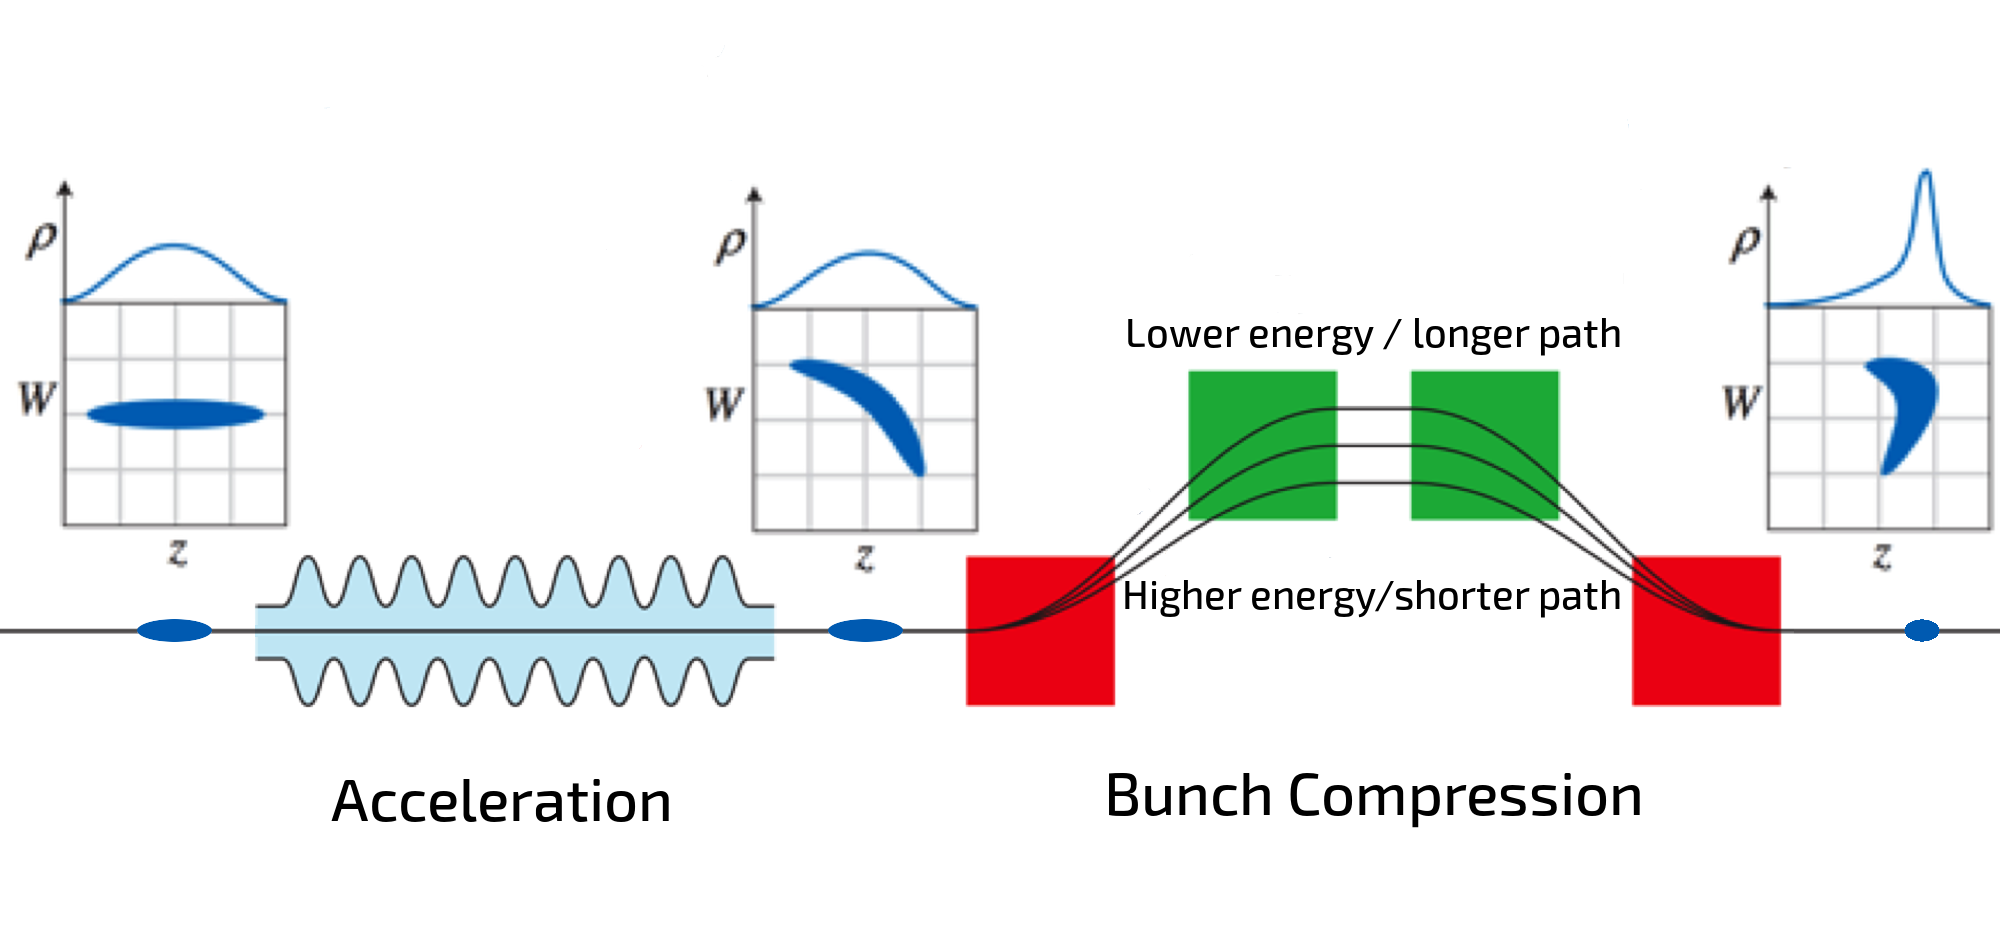
\includegraphics[width=100mm]{Chapter_03_Acceleration_v2.png}
\caption{Schematic of acceleration and bunch compression at LCLS. a-c) change of bunch shape throughout the accelerator. d) illustration of the off-crest accelleration principle. a) shows that this creates an energy chirp. e) schematic of a single klystron. f) schematic of a chicane. The green and red blocks represent magnetic dipoles that deflect the electron bunch in the opposite direction. The path of high energy electrons diverges less than lower energy electrons. If the bunch has a negative energy chirp, this results in bunch compression.}\label{fig:AC}
\end{figure}

\subsection{Bunch Compression}
Short and compact bunches are essential for an XFEL. The main bunch-compression devices are chicanes. Chicanes consist of four magnetic dipoles that cause the high energy part of the bunch to deflect less than the low energy part (see Figure \ref{fig:AC} ). Due to the negative energy gradient it thus reduces the temporal spread of the bunch. After the final compression the electron bunch is ~40 fs long. Creating these short bunches is a noteworthy technical achievement.


The intensity of this radiation scales with the number of electrons in the bunch. Photons co-propagate with the relativistic electrons and if the undulator is long enough, induce an energy modulation, leading to a periodic density modulation in the electron cloud. The resulting microbunches behave like giant charged particles, and emit photons proportional to the square of their total charge in the undulator. At wavelengths longer than the bunch length, this radiation is coherent. This phenomenon of self-amplified spontaneous emission (SASE) is exploited to create powerful X-ray free-electron lasers, using very long undulator structures.




\section{Undulator}
After the acceleration the electron bunches are sent through a periodic arrangement of magnets with alternating poles called an undulator. The magnetic field in the undulator is given by:
\begin{equation}\vec{B}(z) = B_0\cos{(\frac{2\pi}{\lambda_u}z)}\hat{\mathbf{y}}\label{eq:bz}\end{equation}
where $B_0$ is the magnetic field and $\lambda_u$ is the length of an undulator period.
Due to the magnetic field the moving bunch of electrons experience a Lorentz force, causing it to oscillate in the transverse direction (x). The movement can be described by the following equation. 
%\begin{equation}\vec{F} = e(\vec{v}\times\vec{B})\end{equation}
\begin{equation}v_x = \frac{-e\,B_0\,\lambda_u}{2\pi\,m_e\gamma} \sin{(\frac{2\pi}{\lambda_u}z)} = \frac{K c}{\gamma} \sin{(k_uz)}\label{eq:vx}\end{equation}
The non-dimensional parameter K is given by:
\[K =  \frac{-e\,B_0\,\lambda_u}{2\pi\,m_e \, c}  \approx 0.9337 B_0 \lambda_u\]
where the approximation is valid when the magnetic field is given in Tesla and the undulator period in centimeters.

To preserve momentum during the oscillation, the electrons emit radiation with a wavelength $\lambda_s$. As described in Chapter 2, interference effects will occur between the emitted waves from the different electrons. The essence of this interference phenomenon lies in the longer route taken by the oscillating electrons compared to the radiation, which causes an OPD between the radiation emitted by electrons one undulator period apart. If the OPD between the electrons and the radiation is equal to a multiple of $\lambda_s$, the emitted waves will add coherently. Radiation with other wavelengths will interfere destructively. The longer an undulator, the more pronounced will this selection of specific wavelengths be. Equation \ref{eq:res} describes this so-called resonance condition.%, as shown in figure 3b.
\begin{equation}c\frac{\lambda_u}{\langle v_z \rangle } -\lambda_u\, \cos{(\theta)} = n \lambda_s \label{eq:res}\end{equation}
To predict at which wavelength this happens we need to find the average longitudinal velocity $\langle v_z \rangle$. Since the total speed, $v$, of the electrons is not affected by the Lorentz force, the longitudinal speed is calculated using pythagoras theorem: $v_z = \sqrt{ {v}^2-{v_x}^2}$. Using Equation \ref{eq:vx} for $v_x$ and $\gamma^2 \equiv (1-\frac{v^2}{c^2})^{-1}$, we can write $v_z$ as: 
\[ v_z = \sqrt{c^2(1-\frac{1}{\gamma^2})-\frac{K^2 c^2}{\gamma^2}\sin^2(k_u\,z)} = c \sqrt{1-\frac{1}{\gamma^2}(1-K^2\sin^2(k_u\,z))}\]
Using the mathematical identity $\frac{1}{\pi}\int_{0}^{\pi} \sin^2( x ) \, dx =\frac{1}{2} $, integrating of half a undulator period gives the average velocity $\langle v_z \rangle$.
\[ \langle v_z \rangle = c\sqrt{1-\frac{1}{\gamma^2}(1-\frac{K^2}{2})}\]
Assuming that ${\gamma} \gg 1$ we can expand the square root using a first order Taylor expansion: $\sqrt{1+x} = 1+\frac{1}{2}x-\frac{1}{8}x^2+ ...$.
\[\langle v_z \rangle \approx c(1-\frac{1}{2\gamma^2}(1+\frac{K^2}{2}) )\]
If we now assume that we only observe the radiation in the forward direction, we can expand $\cos{(\theta)} = 1-\frac{\theta^2}{2}$. 
Equation \ref{eq:res} can thus be written as:
\[ n \lambda_s = \lambda_u[\frac{1}{1-\frac{1}{2 \gamma^2}(1+\frac{K^2}{2})} - (1-\frac{\theta^2}{2})]\]
We then simplify the first fraction by recognizing that it is given by the geometrical series $\frac{1}{1-x} = 1+x+x^2+...$.By approximating it to the first two terms we are left with the so-called undulator equation.
\begin{equation}\label{eq:undulator}
n \lambda_s = \frac{\lambda_u}{2 \gamma^2}(1+\frac{K^2}{2}+(\gamma\theta)^2)
\end{equation} 

This formula can be explained by two relativistic effects. For an observer it is the electron bunch that is moving at close to the speed of light. In frame of reference of the electron bunch it is however the undulator that is moving very fast. Fast objects are length contracted, thus the electrons observe an undulator period that is contracted to  $\frac{\lambda_u}{\gamma}$, which makes it emit radiation with wavelength around $\frac{c\lambda_u}{\gamma}$. The radiation is in turn relativistically contracted by the relativistic doppler effect when observed in the laboratory's frame of reference, which adds the second gamma term in equation \ref{eq:undulator}. The size of the relativistic doppler effect is dependent on the angle of observation relative to the direction of motion. This will cause a concentration of the energy in the forwards direction where the doppler shift is the largest.

The final wavelength of the emitted light is thus dependent on the energy of the electrons ($v$), the magnetic field in the undulator ($B$), and the angle of observation ($\theta$). Control over these variables makes the selection of a specific wavelength possible. 

%\subsection{Direction of Emission}
\section{Self-Amplified Stimulated Emission (SASE)}
So far in this explanation the electrons produce synchrotron radiation enhanced at specific wavelengths. The intensity of this radiation scales with the number of electrons in the bunch, as the radiation is not temporally coherent. The emitted photons however co-propagate with the relativistic electrons and if the undulator is long enough, the electric field of the radiation will induce an energy modulation within the electron bunch (See Figure \ref{fig:microbunching}. The resulting microbunches behave like giant charged particles, and emit photons proportional to the square of their total charge in the undulator. At wavelengths longer than the bunch length, this radiation is coherent. This phenomenon of self-amplified spontaneous emission (SASE) is exploited to create powerful X-ray free-electron lasers, using very long undulator structures \cite{Kondratenko1980, Bonifacio1984}. 

\begin{figure}[h]
\centering
\includegraphics[width=100mm]{Chapter_03_GenerationXrayXFEL_microbunching.png}
\caption{Self-samplified stimulated emission (SASE). The electric field of the radiation will induce an energy modulation within the electron bunch, that results in microbunches. The three panels illustrate that the electric field will induce an energy modulation within the electron bunch. Certain electrons will be accelerated, and others decellerated, as indicated by the green and red areas. This phenomenon is called slippage. As a result the electrons group in microbunches. The modulation amplifies as more and more electrons group together. The amplications will end when all electrons emit in phase.  }\label{fig:microbunching}
\end{figure}
    \chapter{Substrate-free sample delivery}
In FXI everything that is illuminated by the X-ray pulse is sample. In the case of weakly scattering single particles scattering from any substrate around the might drown the signal from the particle itself. Aerosol injection removes this clutter and assures that the sample is clearly isolated from its surroundings, and this, as we see in a later chapter 6, is important for image recovery.

An aerosol injector produces small droplets of particles dissolved in a volatile buffer. The buffer evaporates under the reduced pressure inside the experimental chamber, ideally leaving behind only the particle. There are two main types of nozzles that can be used to produce small drops: the Gas Dynamic Virtual Nozzle, and electro spray ionisation (ESI).

\begin{figure}[h]\label{fig:drop_formation}
\centering 
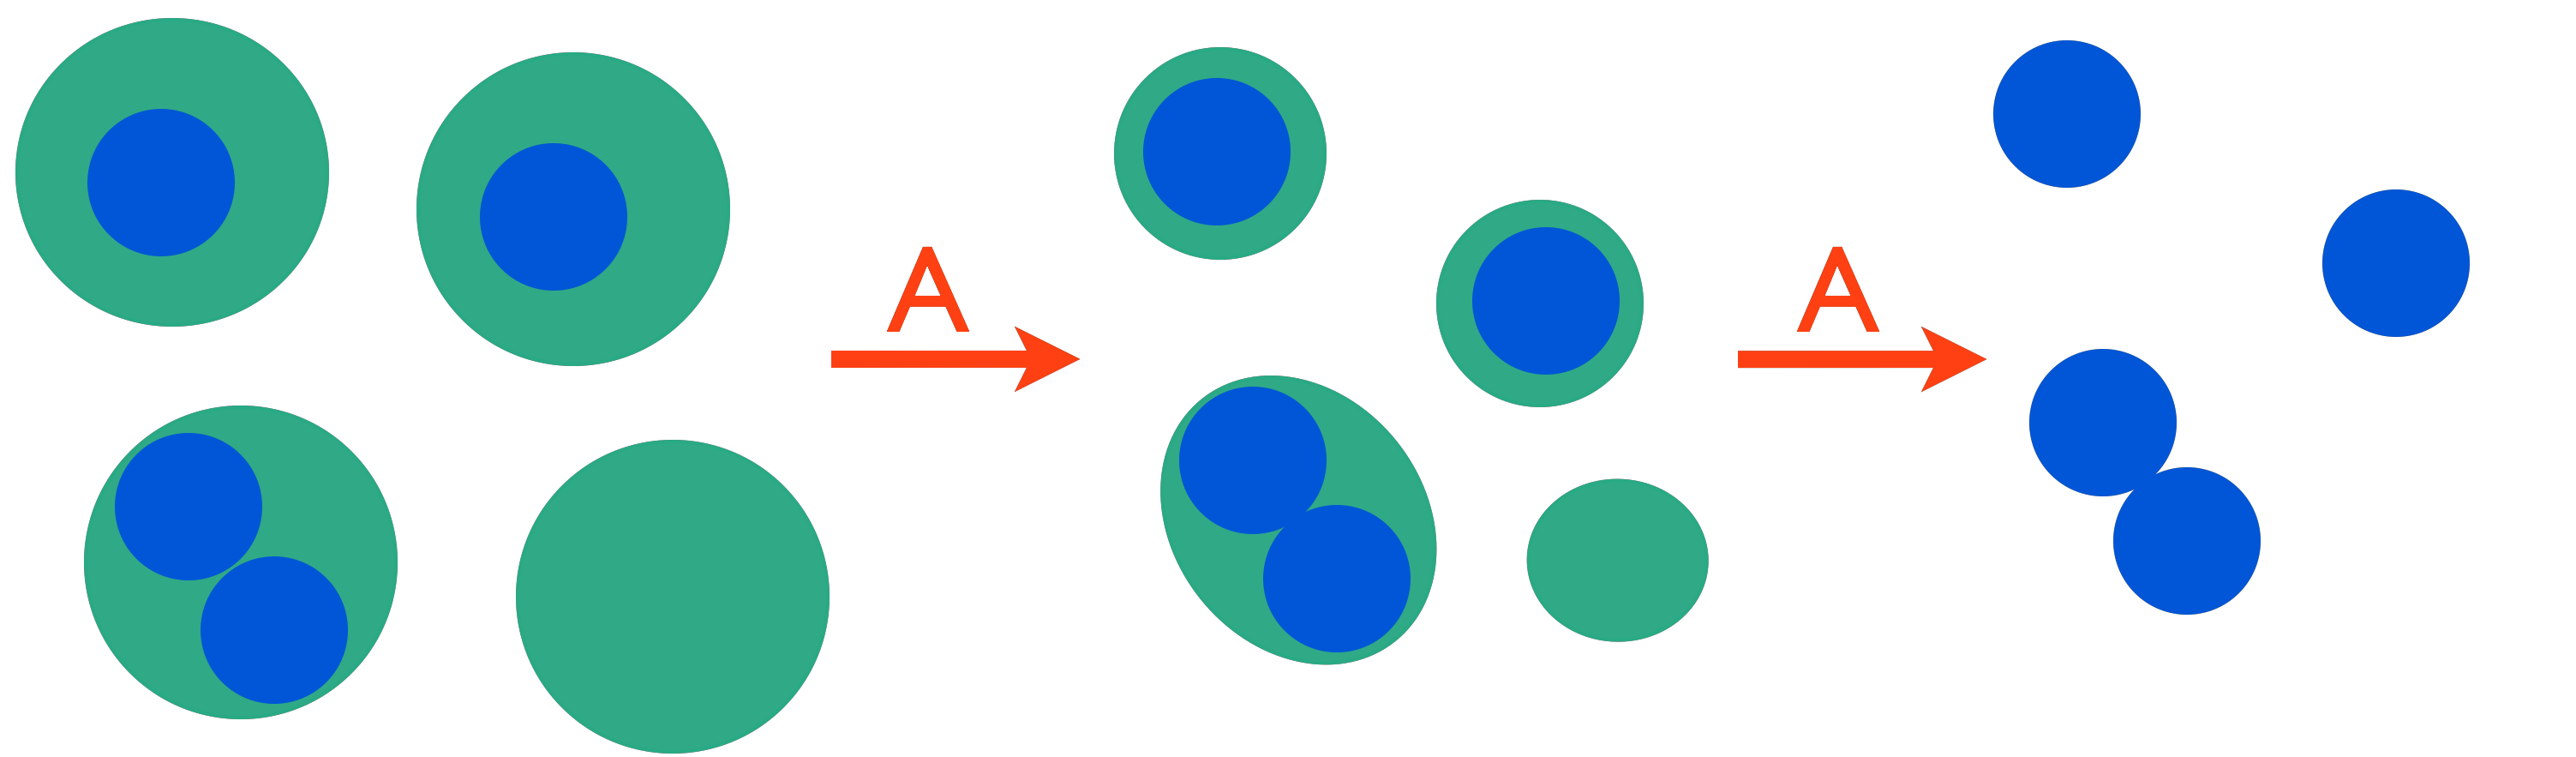
\includegraphics[width=120mm]{Chapter_04_GDVNEvaporation.png}
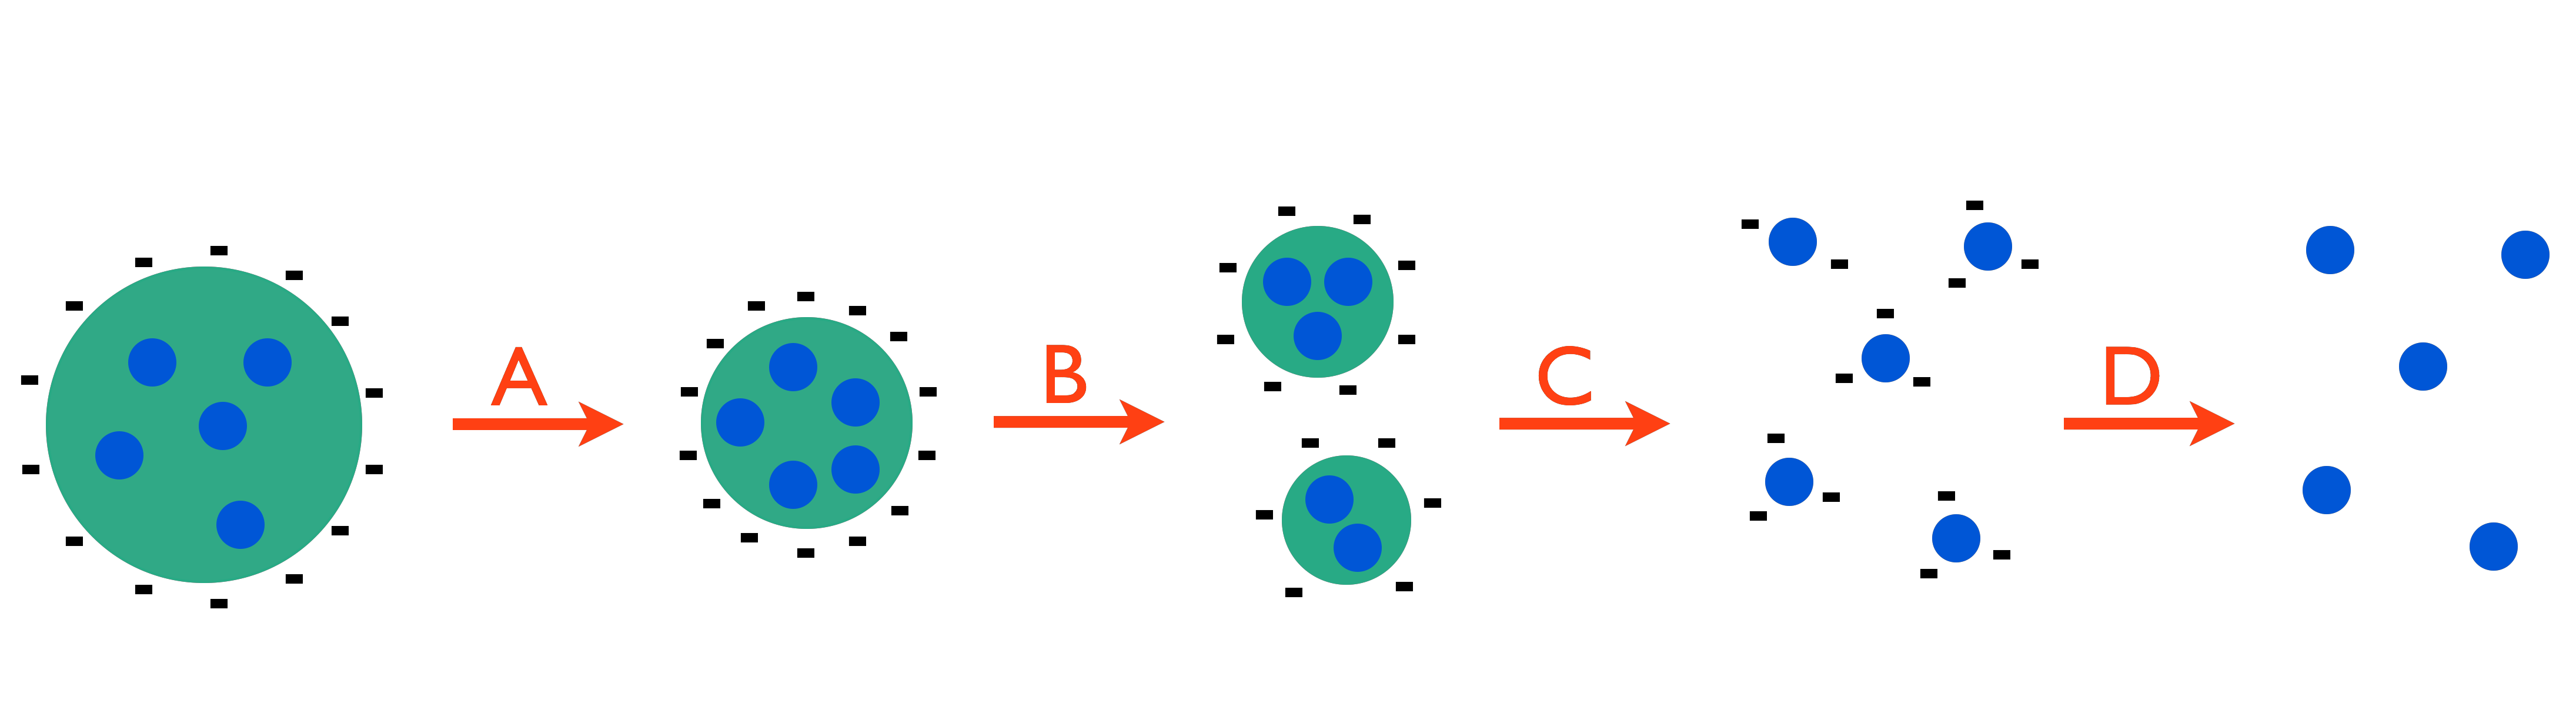
\includegraphics[width=120mm]{ESI_drop_evaporation_explosion.png}

\caption{Experimental geometry, including different sample delivery system. From the bottom left the x-rays pulses enter the chamber. The experimentalist can now select a sample delivery system. Shown are an aerosol sample delivery system, liquid jet injection system, and two types of substrate bound sample delivery systems. If the beam intersect the sample (and/or substrate) a diffraction pattern is recorded on two sets of detectors, placed at different distances from the interaction region.}
\end{figure}




\subsection{Gas Dynamic Virtual Nozzle}

If the coaxial flow of gas creates a jet with a diameter smaller than then a characteristic $d_j$ the surface tension in the liquid will cause the jet to break up into a mist of small droplets. $d_j$ can be estimated on the basis of energy conservation, and is a function of the effective pressure drop $\Delta P$. It is assumed that all energy is transformed to kinetic energy \cite{Acero2013}.
\begin{equation}
d_j^{(GDVN)} = 2 \sqrt{Q \cdot \left(\frac{\rho}{2 \pi^2 \Delta P}\right)^{1/2}}
\end{equation}    
$Q$ denotes the flow rate and $\rho$ is the density of the liquid. The final drop diameter $d_d$ can be related to the jet diameter using the ratio $d_d / d_j \approx 1.9$, which is the classical Rayleigh breakup []. Empirically this assumption has been shown to work well for low-viscosity media such as water. The GDVN can create droplets in the size range of 400 nm - 2000 nm. Sample consumption is in the range of ul/min.

\subsection{Aerodynamic Lens Stack}
After the droplets formed, they start to evaporate in the reduced pressure environment, leaving only the non-volatile particles in the 'drop'. The aerosolised particles are guided into an aerodynamic lens stack (see figure ). This is a series of cylindrical cavities, connected by co-aligned orifices, that collimate the droplets into a narrow beam of particles [].

\begin{figure}[h]\label{fig:skimmer_aerolens}
\centering 
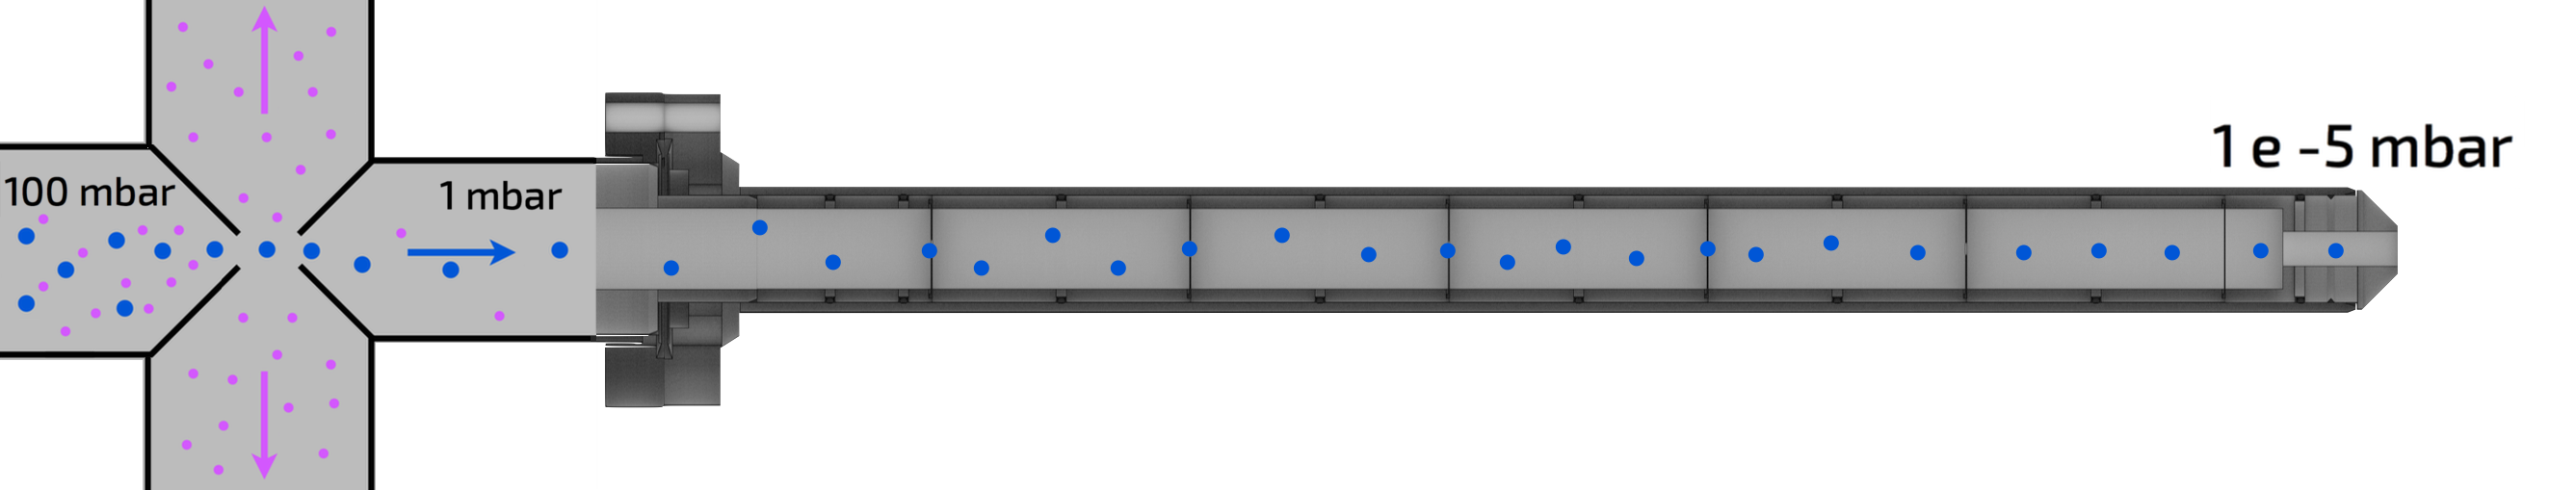
\includegraphics[width=120mm]{Chapter_04_SkimmerAerodynamicLens.png}
\caption{Experimental geometry, including different sample delivery system. From the bottom left the x-rays pulses enter the chamber. The experimentalist can now select a sample delivery system. Shown are an aerosol sample delivery system, liquid jet injection system, and two types of substrate bound sample delivery systems. If the beam intersect the sample (and/or substrate) a diffraction pattern is recorded on two sets of detectors, placed at different distances from the interaction region.}
\end{figure}

For robust particles, which are large compared to the drop size, this type of sample injection has proven to be very successful. This sample injection method made it possible to measure the diffraction patterns from isolated single particles at high signal-to-noise ratios at very high repetition rates. Up to 80\% hit rates have been recorded with a 120 Hz repetition rates at the LCLS \cite{Hantke2013}. The results discussed in this thesis come from datasets that were generated using the GVDN injection method.

For many samples aerosol injection is not disruptive. Molecular dynamics simulation have shown that the conformation of proteins is conserved up till the moment that the last structural water evaporates[]. For the cyanobacterial cells described in this paper it has been shown that the shape and the autofluorescence properties of the cell membranes of the injected cells remain unchanged [PAPER I]. This is not quite unexpected. Aerosols of cyanobacteria can be carried for long distances, and metabolically active cells have been detected at altitudes of 20-70 km where atmospheric pressure drops to below a millibar []. Other sample cell lines such as \textit{E. coli} and brewers yeast, and many types of viruses have been shown to be viable after injection. Nevertheless, not all sample types may be amenable to aerosol sample injection, and samples should be tested prior to experiments.  

\subsection{Electro Spray Ionisation}
Over the last years it became apparent that GDVN sample injection does have its limitations. If the particle becomes small compared to the drop size, wide size distributions of otherwise uniformly sized particles were measured [Daurer, Hantke]. These observations might be explained by a combination of an incomplete evaporation process, and the build up of a significant shell of debris, originating from impurities present in the solution, around the particle. To purify the measured sample, smaller drops had to be generated. A common aerosolisation technique used in mass spectrometry called electro spray ionisation (ESI) is known to be able to produce small droplets.

ESI nozzles produce droplets through a similar droplet formation process as occurs in the GDVN. The difference lies in the process that drives jet acceleration. In ESI the jet is accelerated by an externally applied electrostatic potential. In the capillary the solvent (volatile buffer) is mixed with negatively charged ions. By applying an external field these ions are accelerated, accelerating the entire jet. The accelerated jet will ultimately break into small drops similar to what occurs in a GDVN. The characteristic $d_j^{ESI}$ can be described as a function of the surface tension $\sigma$, vacuum permittivity $\varepsilon_0$, electrical conductivity $C$, as well as the flow rate and the density of the liquid.
\begin{equation}
d_j^{(ESI)} \approx 2 \sqrt{Q \cdot \left(\frac{\rho \varepsilon_0}{\sigma C}\right)^{1/3}}
\end{equation}

After the process of evaporation initiates, an electric potential further builds up in the drops, eventually leading to a Coulomb explosion of the drops [Cole]. Cycles of evarporation and explosion leads to smaller and smaller drops. Initial experiments showed that drops of mono disperse droplets of size 150-200 nm can be generated with ESI. ESI can also be combined with an aerodynamic lens stack. 

The transfer of ESI to FXI is a considerable achievement that will allow the field to move forward to image smaller particles such as proteins. This would not have been possible using the GDVN aerosolisation. ESI has been shown to also function under lower flowrates, reducing sample consumption to 10 nl/min []. This sample consumption rate is advantageous for samples that are only available in small quantities. 

\subsection{Drop-on-demand}
The combination of ESI and a quadrupole with an ion trap for storage allows for a pulsed delivery system that can be tuned to match the repetition rate of the XFEL. This is generally referred to as drop-on-demand. This would reduce the sample consumption even further. Moreover the ion trap can also be utilized for sample selection prior to injection of sample into the x-ray pulse. This is important for single proteins as they scatter very little signal, which makes it very difficult to separate the diffraction patterns from the particle-of-interest and those diffraction patterns obtained from contaminating particles or other noise. 


    \chapter{Data recording}
As we have learned in Chapter 2, a diffraction pattern is the Fourier transform of the scattering potential, sampled at the Ewald sphere ($F({\vec{S}})$). This Chapter will describe the essentials of the process of measuring the diffracted signal.

The value of $F(\vec{S})$ is complex. The complex amplitude corresponds to the amplitude of the measured wave, and the complex argument corresponds to the phase shift of the wave. Currently no device exists capable of measuring the phase of x-rays directly, as it changes in the attosecond time range. The amplitude of the electron magnetic wave can be determined, and this is exactly what is recorded in an intensity measurement. 

\begin{equation}
I(\vec{S}) = |F(\vec{S})|^2
\end{equation}
where $I(\vec{S})$ is the measured intensity.

In the experiments described in this thesis we used a pnCCD detector to determine the $I(\vec{S})$. A pnCCD is a 2D array of pixels of size $p$. Each pixel registers the intensity of the electro magnetic wave at that location by converting the energy present in the wave into an electrical current, using a physical process called the photo-electric effect. 

Figure \ref{fig:experimental_geometry} shows the general setup of a diffraction pattern. There are two pairs of pnCCD detectors. One pair is closed and is placed furthest away from the interaction region. Another detector pair is placed closer to the interaction region, and is opened such that it does not shadow the back detector pair. Figure \ref{fig:experimental_geometry} also shows an aerosol injector, as this is the injection method most used in the experiments described in this thesis.

\begin{figure}[h]
\centering
\includegraphics[width=90mm]{Geometry2.png}
\caption{The experimental geometry. Sample is introduced into the X-ray pulse train, using an aerosol sample injector. The diffracted signal is recorded on two pairs of detectors. The front detector pair is opened such that it does not shadow the back detector. The direct beam passes trough a central hole in the back detector.}\label{fig:experimental_geometry}
\end{figure}

$F(\vec{S})$ is independent from detector distance $d$, while a diffraction pattern is not. The relative scaling factor between the two is $\frac{1}{\lambda\,d}$. This means that the area covered by a pixel of size $p$ on the detector covers an area of size $q = \frac{p}{\lambda \, d}$ of the Ewald sphere (given the small angle approximation holds). 

Using the scaling relation between $F(\vec{S})$ sampled at the Ewald sphere, and the measured diffraction pattern at the detector, we can derive that pixel $P$ on the detector corresponds to pixel $\vec{Q} = \frac{\vec{P}}{\lambda\,d}$ on the Ewald sphere. 

Since $F(\vec{S})$ is measured at discrete locations, we have to use the discrete Fourier transform (DFT), and its inverse, to describe the relation between the measured diffraction pattern and the scattering potential. From now on we will use $F(\vec{Q})$ to describe $F(\vec{S})$ measured at discrete positions. 

The use of the DFT implies that the scattering potential is also discretized. The pixel size in real space (scattering potential space) $r$ is the inverse of the size of the detector in Fourier space ($D$). $D = n\,q$, where $n$ in the number of pixels on the detector, $q$ is the size of a pixel on the Ewald sphere. $q$ is the scaled version of a detector pixel: 
\begin{equation}\label{eq:q}
q = \frac{p}{\lambda d}
\end{equation}
This makes $r$:
\begin{equation}
r = \frac{\lambda\,d}{n\,p}
\end{equation}
Here $\lambda$ is the wavelength of the radiation, $d$ the detector distance, and $p$ is the size of a detector pixel.

%In a measurement the energy of a EM wave appears quantized, which means that one will always measure an integer number of the basic quantum of radiation: photons. The energy of a photon is related to its wavelength. The quantisation the measured intensity also has as an effect on the statistics, as they ar

\section{Missing Data}
The geometry of the detectors used in the experiments described in this thesis consist of two moveable halves (38.4 mm by 76.8 mm), with a dead area of at least 0.8 mm in between both halves (see figure \ref{fig:experimental_geometry}). In the center of the
detector a hole is created to let the high-intensity direct beam through (each detector half misses a semicircle). For both the dead area, and the central hole no intensity information is present, and the diffraction pattern is incomplete. 

In some experiments two pairs of detectors are used, in which one pair located closer to the sample (see figure \ref{fig:experimental_geometry}). The back detector is closed, and the front detector is opened such that it does not shadow the back detector. This opening results in a large area of missing data.
 
\section{Saturation}
Besides missing data due to the detector geometry, detector saturation might also lead to missing information. Each pixel on the detector can maximally hold a certain amount of electrical charge. If more charge is present in the pixel, the excess charge will overflow to neighbouring pixels, making it impossible to accurately use the original pixel as well as the affected pixels. If the amount of charge is very high, saturation might even damage the detector itself. Saturation usually occurs in the center of the detector, because these regions are typically the most intense regions of a diffraction pattern. 





    \chapter{Phase Retrieval}
%As discussed in the previous chapter, the wavefront of the x-ray radiation is described by its amplitude and its phase. As there currently there exists no device capable of measuring the phase of x-ray radiation, in general there is no direct way of recovering the object from the measured diffraction pattern. 
The problem with missing phase information is well known and is called the phase problem. There are many ways to overcome it: for example in crystallography, homology modelling or the anomalous scattering of heavy atoms is exploited to retrieve phases \cite{Rossmann1972,Arndt1978}. In Fourier holography the interference between two wave fields is used to obtain the phases \cite{McNulty1992, Eisebitt2004, Marchesini2008}. In ptychography the precisely known overlap and high redundancy between many exposures is used to solve the phase problem \cite{Rodenburg2007,Thibault2009}. In FXI the scattered field becomes oversampled, which means that, under certain conditions, phases can be retrieved from the intensity pattern itself. The next sections will describe oversampling in more detail, and explain how phases can be retrieved from an oversampled signal using iterative phase retrieval methods, and finally explain how phase retrieval can be validated. 

\section{Oversampling} 
In 1952 Sayre noticed, the Bragg peaks sample the molecular transform $\mathcal{F}(\rho)$ at the critical sampling rate ($\Pi_C$)\cite{Sayre1952a, Shannon1949a}\footnote{It was Bernal \cite{Bernal1938} that already noticed that the signal in between Bragg peaks could be sampled by hydrating and drying crystals.}. This means that if we know the phases in addition to the amplitudes at only the Bragg peaks, it is just enough to back-calculate the structure of the measured object. Single-particle imaging is free from the crystal lattice, and we obtain a continuous diffraction pattern. By choosing the detector distance appropriately such that individual pixels cover a small enough angle, we can sample the molecular transform more finely than the critical sampling rate. This sampling condition is called oversampling. Figure \ref{fig:sampling} illustrates both cases of sampling. 

\begin{figure}[h]
	\centering 
		\includegraphics[width=120mm]{Chapter_06_Sampling.png}
	\caption{Illustration of critical sampling (top row) versus oversampling (bottom row). The right column shows two plots with an 1D signal in black. This signal corresponds to the molecular transform (MT) of our object. The MT is sampled at the critical sampling rate (top left), and an oversampling rate (bottom left). This is indicated by the red and the blue dots, respectively. The middle column shows what the measured signal, associated with the sampling rate, would look like. This bares resemblance to what is measured by a pnCCD. The right most column shows the DFT of both measurements. Important to note is that both DFTs show an similar reconstruction of the original object, but the size of the object compared to the field of view is different. The recovered object is exactly the size of the field of view when the molecular transform is sampled at the critical sampling rate. The size of the object is smaller than the field of view when the molecular transform is oversampled. Oversampling results in zero density around the recovered object.}
	\label{fig:sampling}
\end{figure}

If the oversampling is large enough the redundant information given by the extra sampling point is enough to retrieve the missing phases. The linear sampling rate $R_S$ is defined as the ratio between the actual sampling rate and the oversampling rate.

By choosing a detector setup such that the sampling rate is at least twice as high as the \cite{Bernal1938, Shannon1949a} the critical sampling rate we can use the additional intensity information to recover the missing phases, and thus reconstruct the object from the measured intensities alone. It has been proven that this method often has multiple solutions when applied to 1D data \cite{Walther1963}, however, for higher dimensions it does, in most cases, have a unique solution\cite{Bruck1979}. Oversampling is the basis of many phase retrieval techniques in single particle imaging, as well as some clever phasing techniques applied to Serial Femtosecond X-ray Crystallography (SFX) \cite{Ayyer2016,Chapman2011}.

\section{Iterative Phase retrieval}
In practice there are many ways to possibly retrieve the phase information from the diffraction pattern, but most common phase retrieval techniques are variations of convex optimization algorithms. This section introduces the general idea behind convex optimization, and explains three different algorithms in more detail.

As with many difficult problems, we start from the things that are known. Figure \ref{fig:sampling} shows that oversampling in Fourier space implies that there is an area  around the object with the size ($l-o$) for which we know the electron density $\rho(\vec{r})$ is zero. This knowledge can be used as a constraint on the possible phases. We know that a correct choice of phases would make the corresponding $\rho(r)$ zero in this area. The area that can contain the sample density  and therefore contains nonzero electron density is called the support $M(\vec{r})$. This constraint is called the real-space constraint. Furthermore, we know that the recovered Fourier amplitudes should agree with the measured intensities. This is called the Fourier-space constraint. 

In 1978 Fienup \cite{Fienup1978} introduced an algorithm called Error Reduction (ER) to solve the phase problem. It was inspired by an earlier algorithm by Gerchberg and Saxton \cite{GerchbergSaxton1972}, but applied to the phase problem. ER is an iterative approach that tries to find a solution that minimizes the disagreement with both the real-space constraint and the Fourier constraint. In words it can be described as follows:\\
\begin{enumerate}
\item Assign random phases to each pixel in Fourier space.
\item Inverse Fourier transform to get the corresponding real space.
\item Set all electron density outside the support to zero, keep the electron density inside the support unchanged.
\item Fourier transform the new density to get the corresponding Fourier space.
\item Make the recovered amplitudes match the measured intensities. Keep the phases unchanged.
\item Go back to step 2.\\
\end{enumerate}


ER is sometimes able to find the correct solution, but because the problem is not convex it often gets stuck in local minima and does not find the global solution.

In 1984 Levi and Stark realized that the two constraints described above can be interpreted as projections in a multidimensional Hilbert space \cite{Levi1984}. Step 3 will from now on be called the real-space projection $P_r$. The sequence of step 4,5 and 2 will be called the Fourier Projection $P_f$.  In ER $P_r$ and $P_f$ can be defined as follows:
\begin{align}\label{eq:ER}
P_r \rho\left(\vec{r}\right) =& \begin{cases} \rho\left(\vec{r}\right) \quad &\mathrm{if}\,\,
    \vec{r} \in M\\0 \quad & \mathrm{if}\,\, \vec{r} \not\in M \end{cases}\\
P_f \rho(\vec{r}) =& \mathcal{F}^{-1}\left( \frac{\sqrt{I}}{|\mathcal{F}(\rho(\vec{r}))|}\mathcal{F}(\rho(\vec{r})) \right)
\end{align}

The largest difference between the two projections is that the support constraint is convex, while the Fourier constraint is not. An iteration in ER can now been seen as a real-space projection followed by a Fourier projection. A common and flexible way to express one iteration of the algorithm is by the following equation:
\begin{equation}\label{eq:fom}
\rho_{n+1}\left(\vec{r}\right) = \begin{cases} P_f\rho_{n}\left(\vec{r}\right) \quad &\mathrm{if}\,\,
    \vec{r} \in M\\0 \quad & \mathrm{if}\,\, \vec{r} \not\in M \end{cases}
\end{equation}

Two error metrics can be constructed by measuring the change imposed by the respective projection:	the Fourier error, $E_f$, and the real space error,$E_r$. Intuitively, $E_r$ measures how much of the electron density outside the support. $E_f$ gives the difference between the measured and the recovered amplitudes and the square root of the intensities. Mathematically $E_f$ and $E_r$ are defined as:

\begin{equation}
E_r = \left|P_r\rho(\vec{r}) - \rho(\vec{r})\right| = \left(\sum_i\rho_i^2\right)^{\frac{1}{2}}
\end{equation}

\begin{equation}
E_f = \left|P_f\rho(\vec{r}) - \rho(\vec{r})\right| = \left(\sum_{i}\left(\frac{\sqrt{I_i}}{|F(S_i)|}- F(S_i)\right)\right)^{\frac{1}{2}}
\end{equation}
  
\subsection{The Hybrid Input Output algorithm (HIO)}
In 1982 Fienup introduced an algorithm that can escape from local minima, the so-called the Hybrid Input Output algorithm (HIO) \cite{Fienup1982}. To achieve this HIO makes use of a relaxation parameter called $\beta$. An iteration of HIO can be described as follows, using the same syntax as in equation \ref{eq:fom}:
\begin{align}
\rho_{n+1}\left(\vec{r}\right) = \begin{cases} P_f \rho_{n}\left(\vec{r}\right) \quad &\mathrm{if}\,\,
    \vec{r} \in M\\\rho_n(\vec{r}) -\beta P_f \rho_n(\vec{r}) \quad & \mathrm{if}\,\, \vec{r} \not\in M \end{cases}
\end{align}

I consider the $\beta$ parameter in a similar way as the temperature in simulated annealing. If $\beta$ is large the algorithm can escape deeper local minima. Unfortunately this also means that the global minima might be escape as well. If $\beta$ is small HIO will miss fewer minima, but will have greater difficulty escaping from them. As long as a minimum is not perfect ($E_r$ and $E_f$ are both nonzero), HIO will, given enough time, eventually be able to escape.

\subsection{The Relaxed Averaged Alternating Reflections algorithm (RAAR)}
Another algorithm that is often used in the work described in this thesis is the Relaxed Averaged Alternating Reflection algorithm (RAAR). RAAR does not escape all minima but it can escape shallower ones. For high-quality data RAAR seems to find the solution quicker and more reliably than HIO. An iteration of RAAR can be described as follows:
\begin{align}
\rho_{n+1}\left(\vec{r}\right) = \begin{cases} P_f \rho_{n}\left(\vec{r}\right) \quad & \mathrm{if} \,\,
    \vec{r} \in M\,\mathrm{and}\,\rho_n(\vec{r}) \geq -(1+\beta)P_f\rho_n(\vec{r}) \\\
    \beta\,\rho_n(\vec{r}) -(1-2\beta) P_f \rho_n(\vec{r}) \quad & \mathrm{if}\,\, \mathrm{otherwise} \end{cases}
\end{align}

As both RAAR and HIO do not guarantee to end up in the bottom of a minimum, concluding phase recovery with a number of iteration of ER will ensure that the final solution is close to a minimum. This can improve the overall quality of the reconstruction, as shown in \textbf{Paper I}.

\subsection{Other algorithms}
There exist many other phase recovery algorithms (See \cite{Marchesini2007a}). A software package called Hawk \cite{Maia2010} allows users to select and test different algorithms. Hawk is especially powerful as it is fast and gives direct graphical feedback about the reconstruction process. The latter can for example be very useful in determining the correct support size. 

\section{Shrinkwrap}
While HIO and RAAR perform well when the support is well known and follows the shape of the actual object tightly. In practise this information is often not available and phase retrieval can become practically impossible if the support is too large. In 2003 Marchesini developed an algorithm called Shrinkwrap \cite{Marchesini2003} that does not require an \textit{a priori} known support as input, but instead tries to deduce the shape of the support during the reconstruction. After each $n$ iterations the support is updated by applying a Gaussian blur to the real space image and selecting the pixels that have a value above a certain threshold. The general idea is that even with a somwhat inaccurate support, some features will be recovered well, and by using these features the support will become a bit better, which in turn allows for more feautres to be recovered. The algorithm has been very successful for experimental data \cite{Seibert2011}.

\section{Validation}

\subsection{Errors}
The most basic method to assess the difference in quality between two reconstructions is by comparing the respective errors. The reconstruction with lower errors is generally believed to be a more correct reconstruction. This method does however not teach us anything about the biological validity of a reconstruction and is most often only used to exclude clearly failed reconstructions that will have errors that clearly deviate from the successful ones.
 
\subsection{PRTF}
A standard tool to assess the quality of a reconstruction is the phase retrieval transfer function (PRTF). This function measures the variation within a set of independent reconstructions from the same data but different random starting phases. The PRTF can then be used to quantify the resolution of a reconstruction. The underlying assumption is that any feature that is reproducibly recovered is likely to be a true feature, but non-reproducible features are artifacts caused by the particular starting phases. The variation between reconstructions is calculated for each pixel $i$ in Fourier space by adding together all the recovered amplitudes for that pixel and dividing the total vector by square root of the measured intensity for that pixel $v_i = |\frac{\sum A_i}{\sqrt{I_i}}|$. If the value of $v_i$ is close to unity, all reconstructions recovered a similar amplitude for that pixel. The closer $v_i$ is to zero the more difference is there between the individual reconstructions. The most common way to present the PRTF is to plot the radial average of $v_i$. This plot can be interpreted as a measure of reconstruction quality as a function of resolution. A common practice in the field is to quantify the resolution of a reconstruction by the first time the 1D PRTF drops below the ,somewhat arbitrary, threshold 1 / $e$ (See \cite{Seibert2011}). The corresponding resolution is given by the inverse of the distance to the origin. The real-space solution is presented as the average of all reconstructions that are included in the PRTF. In this image, non-reproducible features will be averaged out and only the reproducible features will be left.
 
\subsection{Missing Mode Analysis}
As described earlier, diffraction patterns often lack data in certain regions. Even in the best case the central region will be missing because the direct beam would otherwise damage the detector. The other main sources of missing data gaps between detector tiles and saturation. 

Reconstruction algorithms deal with this missing data by recovering the amplitude as well as the phase for the pixels in these regions. In many cases the missing data does not affect the stability of phase recovery, this is however not true general. To understand when this happens we have to note that the Fourier constraint does not constrain the amplitudes in the missing data area, and the real-space constraint does not limit the electron density inside the support. If there exists an object that can fit inside the support and has a Fourier transform that is zero outside the missing data region, this object would be completely unconstrained. Such an object could be arbitrarily added to the solution without changing how well the solution forfill the constraints and this would mean that there is not unique solution.

In practice completely unconstrained objects do not exist. Objects that fit inside the support and only slightly contribute outside of the missing data region can however exist. We call such objects weakly constrained. In the design of an experiment, or when deciding whether or not to phase an object it is important to predict whether weakly constrained objects exist for that particular data. This analysis is called missing mode analysis and the weakly constrained objects are usually called modes.

The DFT can be represented in matrix form, where each column represents a pixel in real space and each row represents a pixel in Fourier space. Real space and Fourier space will then each be a vector and the transform itself will be a multiplication with the DFT matrix. The elements in the input and output vectors can be rearranged arbitrarily as long as the corresponding rows and columns of the DFT matrix is rearranged in the same way. Here we have rearranged the pixels so that the unconstrained pixels, i.e. the pixels that are in the support or masked out, come first.


\begin{equation}\label{equ:F_split}
  \mathcal{F} = 
  \left(\begin{array}{l|lll}
    \mathcal{F}_{SM} & &\mathcal{F}_{\bar{S}M}& \\\hline
    &&&\\
    \mathcal{F}_{S\bar{M}} & & \mathcal{F}_{\bar{S}\bar{M}} &\\
    &&&
  \end{array}\right)
\end{equation}

In the matrix above the bar indicates the inverse of the support , $S$, and mask, $M$, respectively. We are only looking for objects that only have values in $S$ and minimize the contribution outside the mask. This means that we need to minimize $|\mathcal{F}_{S\bar{M}}\rho|$. A common method to find such objects is singular value decomposition \cite{Eckart1936}. This method decomposes $|\mathcal{F}_{S\bar{M}}\rho|$ into a diagonal matrix $\Sigma$, and two unitary matrices $U$ and $V$. The values in $\Sigma$ are called singular values. The smallest singular values correspond to the most weakly constraint objects, or weakly constrained modes.

\subsection{Hierarchical Clustering}
As the reconstruction process might end up in different solutions, we typically use the Fourier and real-space error to select what particles to keep for the PRTF. The assumption here is that failed reconstructions have higher error scores that the successful ones. 

I conducted a study to test whether this practice actually selects
In \textbf{Paper I} we used the  UPGMA (Unweighted Pair Group Method with Arithmetic Mean) hierarchical clustering method \cite{Sokal1958} to determine the number of structurally different solutions present in the set of reconstructions. The workflow of this method is illustrated in Figure \ref{fig:UPGMA}.

\begin{figure}[h]
	\centering 
		\includegraphics[width=100mm]{Chapter_06_UPGMAClustering.jpg}
	\caption{Flow chart of the UPGMA Clustering algorithm. In the first step of the algorithm, n independent reconstructions (400 in this example) are compared pairwise, pixel-to-pixel to check similarity. Each comparison results in a so called comparison score. The second step is the actual clustering step in which the number of different clusters present in the set of reconstruction is determined. Initially each reconstruction belongs to its own cluster. In each consecutive merging step the two most similar clusters are merged into one cluster. This repeats itself until one cluster remains. Each merge can be given a similarity score using the comparison	scores from step 1. By plotting the similarity scores against the number of clusters, the number of clusters can be determined. We choose the number of cluster by cheking where this plot makes a kink. This is indicated by the green line in the top graph on the right. The bottom plot shows the Fourier-error and the Real-space error associated to each reconstruction, color-coded on the basis of which cluster they belong to. Here we note that there are four outliers and one main cluster. The outliers are clearly failed reconstructions.}
	\label{fig:UPGMA}
\end{figure}

In the first step of this method each reconstruction is compared pairwise to every other reconstruction, pixel-to-pixel. The comparison score associated with each comparison is the normalized scalar product between the pair of reconstructions, after translating them to their optimal fit. 

In the second step of the method similar reconstructions are grouped in clusters. Initially each reconstruction belongs to its own cluster. In every consecutive step the two most similar clusters are merged into one cluster, until in the end only one big cluster remains. For each merge we calculate a similarity score, which is the average comparison score for all reconstruction in the merged cluster. We plot the similarity score of each cluster merge as a function of the number of clusters. The agglomeration step where the plot makes a "kink" is chosen as the number of different clusters that are present in the set of reconstructions. This is a standard way to estimate the number of clusters present in the set of reconstructions. This capability is an advantage of the  clustering algorithm. 

In a 2D plot of $E_f$ vs. $E_r$, color-coded by cluster, it is possible to see whether or not there is a correlation of reconstruction similarity and error score.  In the case that several large clusters remain after applying a real-space error and Fourier-error threshold the clusters have to be examined carefully. If the remaining clusters correlate with the errors we suggest to keep only the cluster with the lowest error. If no correlation is present between score and cluster it is advised to keep all clusters for further evaluation, because otherwise there is a possibility of selecting on similarity, which would negate the validation power of the PRTF.

 
\section{Simulated Phase Contrast Methods}
Once the phase of the diffraction pattern is retrieved, one has complete knowledge of the information encoded in the  wave-field. This total knowledge is powerful, because it allows the emulation of the action of any imaging system for which an associated mathematical transform can be written, regardless of its experimentally feasibility.
For example, differential interference contrast imaging, otherwise known as Nomarski imaging, is experimentally a well-established technique to visualize the changes in phase \cite{Nomarski1955)}. This change can have biological meaning, for example the density inside certain organelles can be higher than the average density in cells. Normarski imaging will give a more pronounced image of the borders of the organelle. For an example see ref \cite{Barty1998}. 

Nomarkski imaging in its simplest form takes a scattered wave-field, say $\psi(x,y,z = 0)$, and then interferes this wave-field with a copy of itself that has been given both a slight transverse displacement ($\Delta x$, $\Delta y$) and a phase shift $\phi_0$. Thus the intensity of the resulting wave-field $F_N$ is \cite{Paganin2004}:
$|\psi(x,y,z=0)+ e^{(i\phi_0)} \psi(x - \Delta x,y - \Delta y,z=0) |^2$, from which one can show (using the Fourier shift theorem) that the transfer function becomes:
\begin{equation}
\begin{aligned}
\begin{split}
T_{DIC}(q_x, q_y, \tau) = 1 + e^{(i(\phi_0 - q_x \Delta x - q_y \Delta y))},\\
\tau = (\phi_0, \Delta x, \Delta y)
\end{split}
\end{aligned}
\end{equation}

In the case of a reconstructed image $\rho(\vec{r})$, the Normarski variant $N$ will look like:
\begin{equation}
N = \mathcal{F}^{-1} T_{DIC} \mathcal{F}(\rho(\vec{r}))
\end{equation}
We have created simulated Nomarski images of the reconstructed cell images shown in the results part.




    \chapter{Three dimensional Reconstructions}
So far we have dealt with two-dimensional diffraction patterns. Although much can be learned from two-dimensional images, a three-dimensional model is essential to understand the function of biomolecules.
From Chapter 2 we know that a diffraction pattern samples a curved slice through the center of the molecular transform of the object. If the same object would be illuminated from different angles, the resulting diffraction patterns together could sample the complete three-dimensional Fourier transform. The approach in which multiple two-dimensional images from different angles of illumination are combined into one three-dimensional image is called tomography.%This chapter will describe what possibilities there exist to recover the three-dimensional structure of bioparticles using single particle FXI. It will start by describing several methods that use o recover structure of particles that are reproducible in shape such as many viruses and rigid proteins, and after that discusses the poss

\section{Reproducible Particles}
In single particle FXI the illuminated particle is completely destroyed by the pulse. To date, it has therefore not been possible to image one particle multiple times using FXI. Some bioparticles however, are structurally reproducible. This means that diffraction patterns originating from different copies sample the same molecular transform, and can thus be combined to form the 3D fourier transform of the object. 

In order to successfully assemble the 3D molecular transform from multiple diffraction patterns, their relative orientations need to be known. Most of the time this information is unavailable as the sample delivery methods do not allow for orientation selection. A variety of reconstruction algorithms have been proposed for recovering the relative orientation of diffraction data, including the EMC algorithm \cite{Loh2009}, the manifold embedding (ME) set of algorithms \cite{Giannakis2010}, common-arc algorithm \cite{Bortel2011}, and multi-particle cross-correlation analysis \cite{Kam1977, Saldin2010, Kirian2011}. Theoretical studies suggest that the determination of diffraction pattern orientation should be possible even with photon counts as little as 100 scattered photons per image \cite{Loh2009}.

\section{The Common Arc algorithm}

Two diffraction patterns of the same object, will sample the same Fourier space. Because both diffraction patterns will slice the Fourier transform through the origin, both patterns must have at least an arc in common. The common arc algorithm uses this knowledge to find the relative orientation between two diffraction patterns. In short this algorithm can be described as follows. For each pair of patterns all possible arcs between the two pattern are compared and the best match is chosen as the true one. Based on the retrieved relative orientations between many pairs of patterns a full 3D model can be assembled. This method is successful as long as the diffraction patterns are not very noisy \cite{Tegze2012}. Too much noise makes the comparison between diffraction patterns unreliable.

\section{The expansion maximization compression (EMC) algorithm}
The expansion maximization compression (EMC) algorithm is an iterative algorithm. In each iteration the measured 2D diffraction patterns ($K_j$), where $j$ is the index of each pattern, are used to update a model of the molecular transform of the object ($M^{MT}$). The starting model can be chosen to be random, or if more is known about the model, this information could be incorporated. 

\subsection{Expand} 

Each iteration starts with the expand step in which the 3D model is expanded in all possible 2D slices throught the center, up to a specified angular accuracy. These slices are denoted $W_k$, where $k$ is the index of each slice. These slices represent the possible diffraction patterns given model $M^{MT}$. 

\subsection{Maximization} 

In the next step, each of the slices is compared to each diffraction pattern. This results in a matrix $R_{j,k}$ that describes how well each diffraction pattern fits in each orientation. The distance metric used for comparing the measured pattern to the predicted pattern often makes use of the noise type that affected the measurement. For instance, if you know that your measurement is only affected by shot noise one could use a Poissonian distance metric:
\begin{equation}
d_{Poisson}(W,K) = \frac{e^{-W_i}W_i^{K_i}}{K_i !}
\end{equation}
Here $i$ indicates the i-th pixel.

If you know your measurement is affected by a source that follows a Gaussian distribution $d_Gaussian$ can be used.
\begin{equation}
d_{Gaussian}(W,K) = e^{-\frac{(W_i-K_i)^2}{2\sigma^2}}
\end{equation}
Here $\sigma$ is the width of the noise distribution. Each slice in the expanded model is then updated by summing up the measured diffraction patterns weighted by the coefficients from $R_{i,j}$. This will localize the patterns to the orientations where they fit best.

\subsection{Compression}

In the final step a new model $M^{MT}$ is generated by putting back to updated slices $W_k$ in their respective orientations. This will enforce that the slices in the next expanded model will be internally consitent with each other.

\subsection{Fluence recovery}

So far we have assumed that the diffraction patterns from reproducible particles sample the same molecular transform. This is true as long as $E_0$, the strength of the x-ray pulse that hit the particle, is the same for each exposure. This we know is not the case (see Chapter 3). Due to the randomness of the SASE process the power of the pulse does fluctuate from shot to shot. Even if the total power of the pulse is known, it is unknown where in the pulse the particle was hit.Fortunately, EMC can also be used to recover this effective strength of the electric field using the following equation \cite{Loh2010}.
\begin{equation}
\Phi(K,W) = \frac{\sum_{j} R_{i,j} \sum_{i} K_{i,k}^2 }{\sum_{j} R_{i,j} \sum_{i} W_{i,j} K_{i,k}}
\end{equation}
This so-called scaling term $\Phi(W,K)$ is calculated each iteration after the maximization step. It is used in the maximization step to scale the diffraction pattern when construction a new model.

%Number of orientations

%According to [] the number of patterns that are required to assemble a model of the molecular transform at resolution $R$, which probability $p$ is:
%\begin{equation}
%N = \frac{ln(1-p^{1/K})}{ln(1-k/K)}
%\end{equation}


It is amazing how much noise EMC can tolerate, and still be able to retrieve orientations. This is true even if the noise model is not accurate. For the success of model assembly, it seems more important for EMC to, initially when the model is far from true, have the option to place diffraction patterns in a wide distributions of orientations, than it is to know the behaviour of the noise exactly.


%\subsection{Multi-model EMC}
%Often biomolecules are not static in their structure, but rather are flexible units, that structurally undergo small local changes, or sometimes even large global changes. So far FXI has not been shown to which means that the diffraction patterns sample the structural variation (or conformational landscape). This gives FXI the large potential of being able to map the conformational landscape of each protein, at room temperature. This makes it impossible to create one single structure from all diffraction pattern. Currently an EMC version is being developed that can be assemble multiple models from the data, and tries to deal with the structural heterogeneity is this way. It is very similar to single state EMC, but differs in the fact that it builds multiple self-consistent models. 
    \part{Results}
\chapter{Computational Results}

\section{Pattern classification using RedFlamingo}
Given the high data rates of XFELs it is impossible for humans to go through all data frames individually, and assistance of computers is needed. I wrote an open-source software framework called RedFlamingo that is designed to rapidly assess individual diffraction patterns by reducing their complexity to a small set of interpretable numbers (https://bitbucket.org/gschot/redflamingo). The power of RedFlamingo lies in its speed and modularity: users have the option to select a combination of algorithms they want to use for data evaluation, and can port their own algorithms. This is important, as each sample and experiment will come with its own set of demands on data analysis. For example the number of scattered photons vary considerably from sample to sample. This will affect the way diffraction patterns can be evaluated. The detector type often changes from experimental station to experimental station, and each experiment has its own specific artefacts due to the experimental condition at the time of operation. Within this variation it is very important to be able to know whether or not you are imaging the particle of interest, at what rate you are collecting usable data, and if the sample is intact. Furthermore, in order for algorithms such as EMC to succeed, the amount of heterogeneity within the selected set of diffraction patterns has to be limited. This chapter will describe the framework of RedFlamingo, as well a few algorithms that I have developed to assess common sources of heterogeneity.

\section{The framework of RedFlamingo}
Figure \ref{fig:workflow} illustrates the workflow of RedFlamingo. As input RedFlamingo uses a set of diffraction patterns, and if the selected algorithms require parameters, these are supplied in a configuration file. This particular workflow made use of eight different algorithms. Five of them evaluate the original diffraction pattern, and three of the algorithm make use of the autocorrelation of the diffraction patterns. Algorithms can easily be added or removed from this list. The configuration file can also be used to turn algorithms on or off. 

The algorithms imported into RedFlamingo can use the results from one and other. For example, the results from the signal-distribution algorithm are used for calculating the filtered autocorrelation (see \cite{Seibert2011}) used in particle shape evaluation. Filtered autocorrelation are  affected by the number of scattered photons. This reduces the number of parameters that need to be known before hand, which aids automated pattern selection significantly.

As output RedFlamingo produces a list of scores for each individual diffraction patterns. The scores can be used for pattern selection. For example, the scores can be used to select the most intense, but non-saturated diffraction patterns coming from particles larger than 500 nm. The selected patterns can be used by other algorithms such as EMC, or parameters such as size or particle shape can be used in automated phasing. 


%This makes it very difficult to design algorithms that are useful for every data set.RedFlamingo will make it possible to combine algorithms from different experiments, each often designed to tackle a specific problem. 


%In order for algorithms such as EMC to work, the amount of heterogeneity within the diffraction data set has to be limited. Furthermore, each of the steps in the experiment introduces its own type of noise to the measured diffraction pattern. For example think of the debris clumping around small particles compared to the drop when sprayed with the GDVN, detector malfunction or saturation, or intensity fluctuations due to the random start of the SASE process. Often the results of the first two types of noise can not be tolerated by EMC, and image classification before the EMC step is necessary. Furthermore, fast feedback about the first type of noise is very useful to have during the experiment. So far a very robust sizing method has been developed, but more extended methods might become useful. Several methods shown here can give rapid feedback on particle heterogeneity.

\begin{figure}[!h]
\centering
\includegraphics[width=80mm]{Chapter_08_RedFlamingo_Workflow.png}
\caption{The workflow of RedFlamingo. RedFlamingo takes a set of diffraction patterns as input. In this particular workflow eigth different algorithms are selected to assess the diffraction data. Five algorithms evaluate the diffraction patterns themselves, and three are assessing the autocorrelation of the diffraction patterns. As an output RedFlamingo produces a list of scores for each diffraction pattern. Based on the scores, certain patterns can be selected (pattern B and D) or disregarded (pattern A and C). }\label{fig:workflow}
\end{figure}
%\section{Template-based classification}
%If your object has a known shape it could be possible to only select the diffraction patterns that are similar to a set of expected diffraction patterns from the object called templates. Paper III explores the possibility of template-based classification. In general this method is highly dependent on the choice of template, as well as the amount and type of variation present in your sample.

\section{Algorithms implemented in RedFlamingo}
A way of selecting diffraction patterns is by extracting general features from the diffraction pattern such as size, particle shape, amount of saturation, and the number of particles in the beam. Based on the relative values associated with the features, individual patterns can be selected or discarded, or if these values are determined during an experiment, the experimental conditions might be rapidly adjusted. This section describes several feature extraction algorithms I have implemented.

\subsection{Size}
A common method to determine the size of an object is fitting the central speckle to the central speckle of simulated diffraction pattern from a sphere. Such fitting is reliable for particles that themself are close to spherical in shape, such as icosahedrally-shaped viruses (\textbf{Paper XVII},\textbf{Paper XIII}). The second minima is, however, not reliable, as the location of this minima depends on the orientation under which an icosahedron is imaged. If the third to the fifth minima are also present in the diffraction pattern, the average of these minima can also be used reliably to determine the size of the object. This method can be especially useful in case the central speckle or first minimum is affected by saturation effects. Figure \ref{fig:sizing} shows the relative reliability of using different minima to assess the size of an icosahedral object. These results come from simulated diffraction patterns \cite{Hantke2016}.

\begin{figure}[!h]
\centering
\includegraphics[width=42mm]{Chapter_08_ImageClassification_Simulated_Icosahedron.png}
\includegraphics[width=65mm]{Chapter_08_ImageClassification_Stats.png}
\includegraphics[width=100mm]{Chapter_08_ImageClassification_Sizing_Results.png}

\caption{Evaluation of the size assessment of a icosahedrally shaped particle of 162 nm, using the location of different minima. a) An example of the simulated diffraction patterns used in this evaluation. Each diffraction pattern has a random orientation with respect to the beam. b) The radial average of the diffraction pattern a) with associated size estimates corresponding to the location of each minima. c) the average size estimates based on the location of the each minima, and their respective standard deviations. Although the first minimum is the best in determining the size of an object by itself, the mean of the 3rd - 5th minima are also very good in determining the size of the object.}\label{fig:sizing}
\end{figure}


\subsection{Edge detection / Assess signal distribution radially}
Some objects can be characterized by having sharp edges. A sharp edge in real space corresponds to a streak in the direction perpendicular to the edge in Fourier space. Objects and/or orientations of objects might be classified by determining if, and how many, streaks are present. Figure \ref{fig:edge_detection} explains the idea behind a streak finding algorithm.

\begin{figure}[!h]
\centering
\includegraphics[width=120mm]{Chapter_08_ImageClassification_Edge_Detection.png}
\caption{An evaluation of where in the diffraction pattern the signal is located. In the first step radial cuts are taken each \textit{n} degrees. In 1) only three cuts are visualized: the blue cut is on a streak, the green one is on the edge of a streak, and the red one is in between two streaks. In step 2 the largest distance from the center where the intensity is above a user-defined thereshold is determined. These points are indicated by the dashed magenta lines in 2). The three cuts from 1) show a difference in signal extend. In step three the maxima in the signal extend are determined (see 3). If a maximum has a 180 degree pair, we consider the pair coming from a streak. The average signal extend is indicated by the lightgreen line. 4) The magenta lines contours the signal extend in the diffraction pattern. The red lines indicates the streak location and the lightgreen circle is the mean signal level.}\label{fig:edge_detection}
\end{figure}

\subsection{Elongation}

It might also be possible to determine the elongation of the particle, either by evaluating the elongation of the central speckle (\textbf{Paper XVII},\textbf{Paper XIII}) or by evaluating the elongation of the central term in a filtered autocorrelation. This is useful in discerning between diffraction from spherical and non-spherical objects. Figure \ref{fig:shape_assessment} shows two diffraction patterns: A and B. Diffraction pattern A originates from a icosahedral object and thus has a round central speckle (CS\_A). The fraction of the shortest distance from the center of the central speckle to the edge of the central speckle (minor) divided by the longest distance is called the elongation $\epsilon_{DP}$. Round central speckles have an elongation of 1. The central speckle of pattern B (CS\_B) is much more elongated. 

The evaluation of the autocorrelations of A and B show a similar result. AC\_A shows a roundish particle, whereas AC\_B shows a density that is more elongated. In the radial average of AC\_A and AC\_B this becomes visible as a mass beyond the maximum. The green area is considered to be part of a round particle, and the red area is considered to be part of an elongated particle. The fraction of the green area divided by the green plus the red area constitutes the elongated parameter $\epsilon_{AC}$. The autocorrelation can only be used for the evaluation of convex objects, as non-convex object might appear roundish. 

\begin{figure}[!h]
\centering
\includegraphics[width=120mm]{Chapter_08_ImageClassification_shape_assessment.png}
\caption{Elongation assessment of the particles that gave rise diffraction pattern A and B. From the central speckles of A and B, CS\_A and CS\_B, have a different shape. The elongation factor $\epsilon_{DP}$ is the fraction of the minor over the major axis of the central speckle. If $\epsilon_{DP}$ is close to 1, the objects that gace rise to the diffraction pattern is considered round in projection. The smaller $\epsilon_{DP}$ the more elongated the particle is considered. The evaluation of the autocorrelation plots show similar results. The central blob in AC\_A is roundish, whereas the central blob is more elongated in AC\_B. In the radial averages of both AC\_A and AC\_B the size of the object is taken as the maximum. The green density is considered part of a spherical object. The red density is considered part of an elongated object. $\epsilon_{AC}$ is the fraction between the green area over the green area + the red area. The closer this fraction is to 1, the more round the particle is considered.}\label{fig:shape_assessment}
\end{figure}


\subsection{The shape of the particle}
An accurate guess for the size of the particle is important for automated phasing. So far automated routines have mainly dealt with icosahedral or round particles, which means the size of the particle, as determined from the central speckle, is enough to determine an accurate support constraint (\textbf{Paper XVII},\textbf{Paper XIII}). The support size and shape of elongated particles such as  cells and many virus species cannot be accurately guessed in this way. Figure \ref{fig:detailed_shape_assessment} illustrates an algorithm that determines the support size and shape of elongated particles by tracing the contour of the central term in a filtered autocorrelation. The algorithm uses Laplace-based edge detection \cite{Mathworks2018}. 

\begin{figure}[!h]
\centering
\includegraphics[width=120mm]{Chapter_08_ImageClassification_Refined_Shape_Assessment2.png}
\caption{Finding the shape of the particle. a) shows the filtered autocorrelation of the particle. b) shows the autocorrelation after applying the laplacean edge detection. c) shows the selected area within the autocorrelation. It matches the central term of the autocorrelation. This shape can be used to determining the major and minor size of the particle, and possibly as a guess for the support size and/or shape. }\label{fig:detailed_shape_assessment}
\end{figure}


\subsection{Multiple scatterers in the focus}

Due to the stochastic nature of the injection method, two particles can end up in the interaction region at the same time. If the particles are attached to each other, a similar pattern to the pattern shown in Figure \ref{fig:shape_assessment} will be measured. If the two particles are, however, separated in space, the scattered signal of the two particles will interfere. As a result so called Newton rings will be observed in the diffraction pattern (see Figure \ref{fig:multiplefinding}). As a result of the interference rings, the autocorrelation will show non-central densities, which are called holograms (see \textbf{Paper X}). By determining the presence of non-central terms in the autocorrelation, it is possible to automatically separate the patterns that have interference rings, from patterns that have not. Figure \ref{fig:multiplefinding} illustrates two different methods for finding the non-central density, the first finds the density in the autocorrelation calculated over the entire diffraction pattern. The second method calculates the autocorrelation of a part of the diffraction pattern (similar to a method described in \textbf{Paper XVIII}).

\begin{figure}[!h]
\centering
\includegraphics[width=120mm]{Chapter_08_ImageClassification_Multiple_Finding.png}
\caption{Assessing the prescence of multiple particles in the focus, located at a distance from each otherFinding the shape of the particle. a) shows a diffraction pattern which has clear circular interference rings present (center of the rings are somewhere beyond the top left corner. Note the gray circular area. This area of the diffraction pattern is used in c). b) shows the autocorrelation of a) after subtraction an average autocorrelation. The subtraction helps to reduce artefacts coming from the missing data. c) shows the autocorrelation of a small circular area in a). Both methods give two peaks.  }\label{fig:multiplefinding}
\end{figure}
    \part{Results}
\chapter{Results}
\section{Imaging live cells}
For the study described in \textbf{Paper I} we used cells of two species of cyanobacteria as a sample: Cyanobium gracile and Synechococcus elongatus. Cyanobacteria are photosynthetic bacteria that can be found in almost any habitat on earth, ranging from hot volcanic areas to cold polar ice caps, and play an important role in the global carbon and nitrogen cycle. In a 25 day cycle an algal bloom of 1000 $km^2$ can sequester around 22,000 tonnes of atmospheric carbon into organic carbon before an infection by cyanophages caused the bloom to collapse.
 
Cyanobium gracile cells were selected for their small size and their robustness with respect to the injection procedure. Solitary C. gracile and S. elongatus cells have an oval-to-cylindrical shape, and vary in size between 0.25-0.4 $\mu$m in diameter and 0.4-4.0 $\mu$m in length [Komarek]. Cells divide symmetrically by binary fission. The two daughter cells separate from each other after reaching the size and shape of the mother cell [Komarek2]. We used non-synchronised cell cultures undergoing active growth providing cells in various stages of their cell cycle. 

The experiments described in \textbf{Paper I} were carried out at the atomic, molecular, and optical science (AMO) endstation at LCLS \cite{Bostedt2013}, at 512 eV (2.40 nm) and 1100 eV (1.13 nm) photon energy.  Figure \ref{fig:ExperimentalSetup} shows the arrangement of the experiment. The length of the photon bunch was about 70 fs. The pulse was focused to a spot of 3 $\mu m$ x 7 $\mu m$. The average photon density in the focus was about $1.1 x 10^{11}$ photons/pulse/$\mu m^2$ at 517 eV, and $8.6 x 10^{10}$ photons/pulse/$\mu m^2$ at 1,100 eV. Far-field diffraction patterns were recorded on a pair of pnCCD detectors \cite{Struder2010} in the CFEL-ASG Multi Purpose (CAMP) instrument \cite{Struder2010}. The detectors were place at 741 mm downstream from the interaction region of the beam and the sample. The detector read out rate matched the 120 Hz repetition rate of the LCLS. 

We collected diffraction patterns of C. gracile cells for 60 minutes at a hit ratio of 43\% and selected the 7,500 clear hits for further analysis, using the Cheetah software package \cite{Barty2014}. The linear sampling ratio of the particle was around 20-fold, which allowed direct phase recovery from the measured intensity patterns. Phase retrieval was not a trivial problem because strong hits saturated the detectors at low diffraction angles. As a compromise, we manually selected medium-strong hits, which contained either no, or only few saturated pixels, while still providing scattered signal to reasonably high resolution. Missing mode analysis revealed no unconstrained modes for all reconstructed cells presented in \textbf{Paper I}. 

Figure  shows the reconstructed exit wave-fronts (images) for six live C. gracile cells together with the corresponding diffraction patterns, and a synthetic Nomarski image. The reconstructions represent 2D projections of the electron density of the cells. The images show the expected morphologies of cells during division [Komarek,Komarek2]. The resolution of each  reconstruction is indicated by the size of the round white dot. Features smaller than the dot need to be interpreted with care.

Phases were retrieved using the Hawk software package. For each pattern 400 reconstructions were made, each starting from different random initial phases. These reconstructions consisted of 5000 iterations with the RAAR algorithm [Luke], using a Shrinkwrap algorithm[Marchesini] for support determination, and concluded with 100 iterations by the ER algorithm[Fienup, Gerchberg-Saxton]. The initial and final support size was selected manually. No additional constraints were used since we anticipated the effects of absorption in the thick cells to give effects similar to a phase object. 

Resolution for the reconstructions was estimated from the PRTF (See Figure \ref{fig:ExperimentalSetup}), using the 1/e cutoff. Before calculating a PRTF and averaging the images we removed outliers among the reconstructions by applying a threshold to the Fourier error. Clustering validates the results from using a threshold on the Fourier-Error and the real-space error(Figures 7 a-j). On average the main cluster contained about 370 out of 400 reconstructions (93\%), except for one case where only 96 reconstructions formed the biggest cluster (Figure 7j). This made us believe that the average image of the main cluster is the true reconstruction minimum. Th failed reconstructions did not find the true minimum.
The scatter plots of Figure 7 a-j show that the real-space error is more reliable than the Fourier-error for identifying failed reconstructions.

Detector saturation limited the achievable resolution.  In fact, the reconstructions shown in Figure \ref{fig:ExperimentalSetup} come from exposures that did not saturate the detectors. A number of much stronger exposures were also recorded, and in some of these exposures the diffraction signal extended to nanometer resolution. Figure \ref{fig:ExperimentalSetup} shows one such pattern for a live S. elongatus cell at 1,100 eV photon energy, 70 fs pulse length, about $10^11$ photons $\mu m^{-2}$ on the sample. Four pnCCD detectors were used to record this pattern (Figure \ref{fig:ExperimentalSetup}b). The configuration of the central back detector in Figure  is identical to the detector used in Figure . The front detector is the same type as the back detector but is placed at 220 mm from the interaction region. In this strong hit, a large part of the back detector was saturated, preventing reliable phasing. The signal however extended beyond 4 nm resolution on the front detectors (at sigma 3.7), which is the size of a small protein molecule. More than 58 million scattered photons were recorded on the back detectors, and 1.3 million on the front detectors. The size of the cell was derived from the autocorrelation. Figure 4c shows that in a log/log representation the drop-off of the signal is linear with spatial frequency in the range covered by our measurements, and the exponent of the signal decay is $-3.31\pm0.01$, matching simulations [Jakobson].

 

\section{Classification}

Sizing diffraction pattern
\\
Sizing Autocorrelation
\\
Identification multiple scatterers
\\	1) Multiple Particles
\\	2) Holographic Images
\\
Edge detection
\\
Particle shape detection
\\	1) Round particles
\\	2) Elongated Particles
\\
Success on wide variety of sizes and scattering strengths.
\\
Template-based Classification
\\

\section{Software}
Given the high data rates of XFELs it is impossible for humans to go through all data frames individually, and assistance of computers is needed.
RedFlamingo is a software framework designed to rapidly assess individual diffraction patterns by reducing their complexity to a small set of interpretable numbers. The power of RedFlamingo lies in its modularity: users have the option to select a combination of algorithms they want to use for data evaluation, and can port their own algorithms. This is important, as each sample and experiment will come with its own set of demands on data analysis. For example the number of scattered photons vary considerably from sample to sample. This will affect the way diffraction patterns can be evaluated. Furthermore, the detector type often changes from experimental station to experimental station, and each experiment has its own specific artefacts due to the experimental condition at the time of operation. Within this variation it is very important to be able to know whether or not you are imaging the particle of interest, at what rate, and if it is intact. For deeper data analysis one often needs to limit the amount of heterogeneity within the data to an even larger extend. This makes is very difficult to design algorithms that are useful for every data set. RedFlamingo will make it possible to combine algorithms from different experiments, each often designed to tackle a specific problem. 

As input RedFlamingo takes a set of diffraction patterns $D$, and a configuration file $C$. The configuration file sets which algorithms should be run, as well as the variables needed to run these algorithms. An example of an input file can be found in Figure \ref{fig:IN_OUT_FILE} Figure \ref{fig:WorkFlow_RF} shows the general pipeline of RedFlamingo, as well as the algorithms currently included into it.


RedFlamingo has been tested on several datasets. This chapter shows three cases that illustrate different demands on the data analysis. In the first example, RedFlamingo is used for pattern classification. The main discriminatory features were size, particle elongation, and number of particles in the beam. The second example shows that RedFlamingo can be used to size particles of a wide range of sizes.  

\subsection{Pattern Classification of heterogeneous RDV data set}
Rice Dwarf Virus (RDV) is the causal agent of rice dwarf disease. It can result in severe crop losses in rice and other gramineae plants in East Asian countries due to stunted growth and chlorotic specks. The structure of RDV has previously been solved to 3.5 $A$ resolution by X-ray crystallography \cite{Nakagawa2003} (PDB 1UF2). RDV is approximately 72 nm in diameter.

Most diffraction patterns in this data set are not affected by detector saturation, which makes it possible to estimate the size of the icosahedral-shaped particle by determining the location of the first minima (see chapter 7).
RDV was classified on the size and shape of the central speckle, and the size and shape of the central term in the autocorrelation. If the central speckle and the central term of the autocorrelation are circular to slightly elongated the particle was classified as a single particle.  

\begin{figure}[h]
\centering
\includegraphics[width=100mm]{Chapter_09_Results_RDV_classes.png}
\includegraphics[width=100mm]{Chapter_09_Results_RDV_size_distribution.png}\label{fig:Classes}
\caption{Classification of particles. Top: one example pattern from each class is shown. The gap between the two detector halves and the beam stop is masked out. Bottom: the size distribution of the 3608 diffraction patterns classified as single hits shows a peak at 63 nm.}
\end{figure}

There are

The second example 
    %\chapter{Outlook}
There exists a conspicuous gap in knowledge about the organisation of life at the mesoscopic level. A technique that potentially can bridge this gap is FXI. The field of FXI is rapidly evolving and many of the initial technical limitation are being solved. For example tools for rapid feedback during experiments have been developed [Daurer], a new injection method has solved an outstanding problem in the delivery of particles smaller than 200 nm in diameter, and EMC is can now deal with conformational heterogeneity. With these developments I am very much looking forward to the first 3D models of a protein, possibly of more than one conformational state. 

This thesis showed progress on the other end of the gap. We show that we have not reached a fundamental limit for live cell imaging with an XFEL. We can introduce living cells in the XFEL beam, and record diffraction patterns at low signal to noise ratios, and hight hit ratios. We recorded scattering beyond 4 nm resolution. With a more powerful X-ray laser sub-nanometer resolution on micron-sized cells should be possible. Image reconstruction has been successful for images that were not affected by detector saturation. The dynamic range of the detector can be extended with the help of a selective attenuator. We have build such a system, and are awaiting beam time. An increased dynamic range will almost certainly extend the resolution of future cell reconstructions. 

An automated reconstruction pipeline for heterogeneous objects is well on its way. The classification of cells on shape, intensity, as well as the exclusion of images affected by artefacts of the experimental procedure have been developed. The underlying algorithms have been combined in a computational framework called RedFlamingo.

In the future machine learning algorithms might be used to correlate small variations in cell structure to for example certain external stimuli, or to general morphological changes such as cell division. One should not forget that we have learned a great deal from projection images, as for example most medical imaging is two dimensional. Using the high repetition rates of XFELs, rare cellular events could be studied for the first time.

RedFlamingo has proven itself to be useful in a wide variety of experiments. As the data and the artefacts within it vary from experiment to experiment, different experiments often require different classification methods. The modular nature of RedFlamingo allowed for easy algorithm selection. It has been successful for pattern selection of small viruses of 70 nm to micrometer sized objects such as cells or giant viruses. RedFlamingo has proven itself also useful for pre-selecting patterns for EMC. This is important because too much sample heterogeneity will cause EMC to fail. Machine assisted pattern recognition might in the future also aid the process of image classification. 

To come back to cell imaging, the most speculative and most interesting question of live cell imaging is: How do we obtain 3D information about the cell and its constituents. The addition of diffraction patterns from non-reproducible objects is very different from the addition of diffraction pattern from reproducible particles, as it results in a phenomenon called incoherent addition. The average diffraction pattern of incoherently added diffraction patterns will look like \cite{Maia2009}:

\begin{equation}
I_{average}(\vec{S}) \propto 2 + 2 cos(2\pi \vec{S} \cdot \vec{r}) e^{-4\pi\vec{S}^2{\sigma_r}^2}
\end{equation}

The cosine term of this equation gives information about the relative position of each electron. This can be interpreted as the structure of the particle. The negative exponential term indicated that the amount of structural information present in the averaged pattern decreases as the variation between the patterns increases. This makes it very difficult to retrieve 3D information from an heterogeneous object such as cells. 

A possible solutions to this problem might lie in a combination of multiple beams and sub-tomogram averaging. Right now it is practically impossible to build two XFELs at different angles. In the future this might be become more feasible as both accelerator and undulator hardware might become much smaller. Moreover, not all beams have to be generated by XFELs, as one high resolution diffraction pattern might be aided by one or more low resolution diffraction patterns produced using a High Harmonic Generation X-ray source for example. The lower resolution diffraction pattern will aid in the elucidation of the third dimension. Using the extra information it might be possible to create a low resolution tomogram of the cell. The strength of the pulses and the number of beams will determine the resolution of the tomogram. One could then select reproducible parts of the tomogram, also known as sub-tomograms, and combing them into a high resolution model of the constituent of that part, possibly in a similar way as currently is implemented in EMC, or done in programs such as pyTOM []. Subtomograms might even come from different cells. Key in this process is identification of the location of the reproducible parts. The high repetition rate and high temporal and spatial resolution obtainable using an XFEL might make it possible to collect enough data to visualize cellular events that occur infrequently, or are short lived. 

, using the curvature of the Ewald sphere to recover information, and using special structures in the XFEL itself.
\subsection{Curvature of the Ewald Sphere}
At high scattering angles it becomes possible to notice the curvature of the Ewald sphere. This is more apparent at longer wavelengths (<400 eV). This curvature can be exploited to resolve 3D information about the object, but the extend at which this is possible is limited. If something is known about the n some cases much is known about the possible shape or buildup of the particle and then it is possible to reconstruct a 3D structure [Miao, Fennel, ...]

\subsection{Structures in the XFEL}
Time structures, multiple wavelengths, highly curved wavefields might make it possible to create a focal plane inside the cell. 

\subsection{Multiple beams and sub-tomogram averaging}
In the future it might be possible to use multiple synchronised X-ray pulses to illuminate cells from different directions. 
	\chapter{Sammanfattning pa Svenska}

In this thesis we want to develop new methods to image biological diversity at the molecular level. Understanding this diversity is very important as it can play a major role in development of deceases. The thesis focuses on two topics: the imaging \textit{living} cells and the development of a computational tool to assess variability within a population of images.
\\\\
In molecular biology structure and function are closely related. This however does not mean that each object has one single static shape. On the contrary, many objects have multiple conformations and only through understanding the variation, their function becomes interpretable. A further complication arises from the fact that the variation is often highly dependent on the exact environment the objects are in. Outside of their natural environment, molecular machines might start operating differently. A tool that could image molecular machinery inside their natural environment, the living cell, is therefore required for us to truly understand the structure of molecular life.
\\\\
The amount of detail we can image in an object is limited to about the size of the wavelength of the light used. Molecular machines are build up out of atoms, so light with a wavelength similar to the size of an atom is needed to see single atoms and thus understand the functioning of molecular machines fully. This type of light is called X-ray radiation. Another fundamental principle is that the smaller an object is, the stronger light is needed in order to record enough information to record an image. Strong beams however have the disadvantage that they damage the objects themselves. This leads to the limitation that single objects smaller than 100 atoms in diameter can not be visualized using ordinary techniques.
\\\\
The development of a new type of X-ray laser called an x-ray free-electron lasers, that produces ultra short and extremely bright X-ray pulses might hold the solution to this limit imposed by sample damage. The power of the pulse ensures that even individual molecular machines can be imaged in atomic detail. These pulses do damage the sample, but because they are ultra-short the damage only happens after the pulse has passed. The recorded image is therefore an image of the undamaged object. This principle is called diffraction before destruction. 
\\\\
The word diffract indicates that we are not recording images of an object in the same way that a photo camera captures images. Instead we measure a so called diffraction pattern. The 2D diffraction pattern can be converted to a real image (2D) in a process called image reconstruction. The feasibility of diffraction before destruction and the image reconstruction process has been shown for a variety of non-biological and biological samples in 2D.  And recently the first 3D model of a biological object has been generated from many diffraction patterns generated using this method.
\\\\
In 2008, researchers showed that it is theoretically possible to image small living cells at sub-nanometer resolution in 2D. The main work of the thesis was an experimental verification of this prediction. This study showed that using an XFEL that was weak compared to the imaginary ones used in the predictions, it is possible to record images with signal up to 4 nm resolution which is equivalent to 40 atomic diameters. The problem of these images is that the strong signal caused the detector to saturate. We therefore had to resort to weaker diffraction patterns for the analysis. This posed the limit on the resolution of the recovered object. We have suggested improvements to avoid detector saturation, but these suggestions have not yet been tested experimentally.
\\\\
Due to the variability between different cells it is not trivial to fully automate the process of object reconstruction from the recorded diffraction, something that is needed to study the variability of cells in high detail, or the molecular machines inside of them. For the automation to succeed it necessary to predict the shape of the object from the recorded image itself. Furthermore, other parameters such as saturation or having two cells in the beam at once also have to automatically identified.
\\\\
To solve this problems I have developed a software suite called RedFlamingo. RedFlamingo can be used to assess the quality of individual images and deduces several essential features for image reconstruction. In some cases it can also determine whether the observed variety originate from a biological source, or whether it is a result from the experiment. It turns out that this feature can be useful in the process of deriving a 3D model from many 2D images. 
\\\\
I am very excited to be part of the development of this technique. Measuring images without saturation effects might open the door to observing the biological processes occurring inside living cells. For the future I see the study of variability in isolated molecular machines as the first milestone. After that I hope that these machines can be studied together with their natural environment, allowing us to visualize the organisation of life.


\backmatter
    % References
    % No restriction is set to the reference styles
    % Save your references in References.bib
    \nocite{*} % Remove this for your own citations
    \bibliographystyle{plain}
    \bibliography{Thesis}

\end{document}